% Chapter Template
\chapter{Cross section measurement} % Main chapter title

\label{Chapter7} % Change X to a consecutive number; for referencing this chapter elsewhere, use \ref{ChapterX}

\lhead{Chapter 7. \emph{Cross section measurement}} % Change X to a consecutive number; this is for the header on each page - perhaps a shortened title


The cross section for the pp$\rightarrow$W+bb+$X$ process is determined separately in the electron and the muon channel using the relation:
\begin{equation}
\sigma = \frac{N_{sig}}{A\times \epsilon \cdot \mathcal{L}}
\label{equ:xsec}
\end{equation}
where $N_{sig}$ is the overall number of the signal events, which is precisely determined by performing the fit procedure presented in the next sections. $A\times \epsilon$ is the detector acceptance and efficiency (section \ref{sec:AE}) and $\mathcal{L}$ is the total integrated luminosity. 
\par Fit methodology is shortly presented in the section \ref{sec:fit}, while the systematic uncertainties, which are taken into account during the fit, are described in detail in section \ref{sec:syst}. The procedure for the calculation of $A\times \epsilon$ is described in \ref{sec:AE}, in section \ref{sec:res} the cross sections results are given and compared to the theoretical prediction. 

%----------------------------------------------------------------------------------------
%	SECTION 2
%----------------------------------------------------------------------------------------

\section{Signal extraction method}
\label{sec:fit}

The Wbb yield is obtained from a fit to the transverse mass distribution recovered after applying the selection criteria described in section \ref{sec:selection}. The fit was performed in the full $M_T$ range to better constrain the QCD contribution.  
The Wbb contribution is modeled using the four-flavor scheme and five-flavor scheme separately, as described in detail in \ref{sec:samples}. The comparison between the two samples is given in figure \ref{fig:4fsvs5fs}. Small differences in shapes can be seen.

\begin{figure}[htbp]
	\centering
		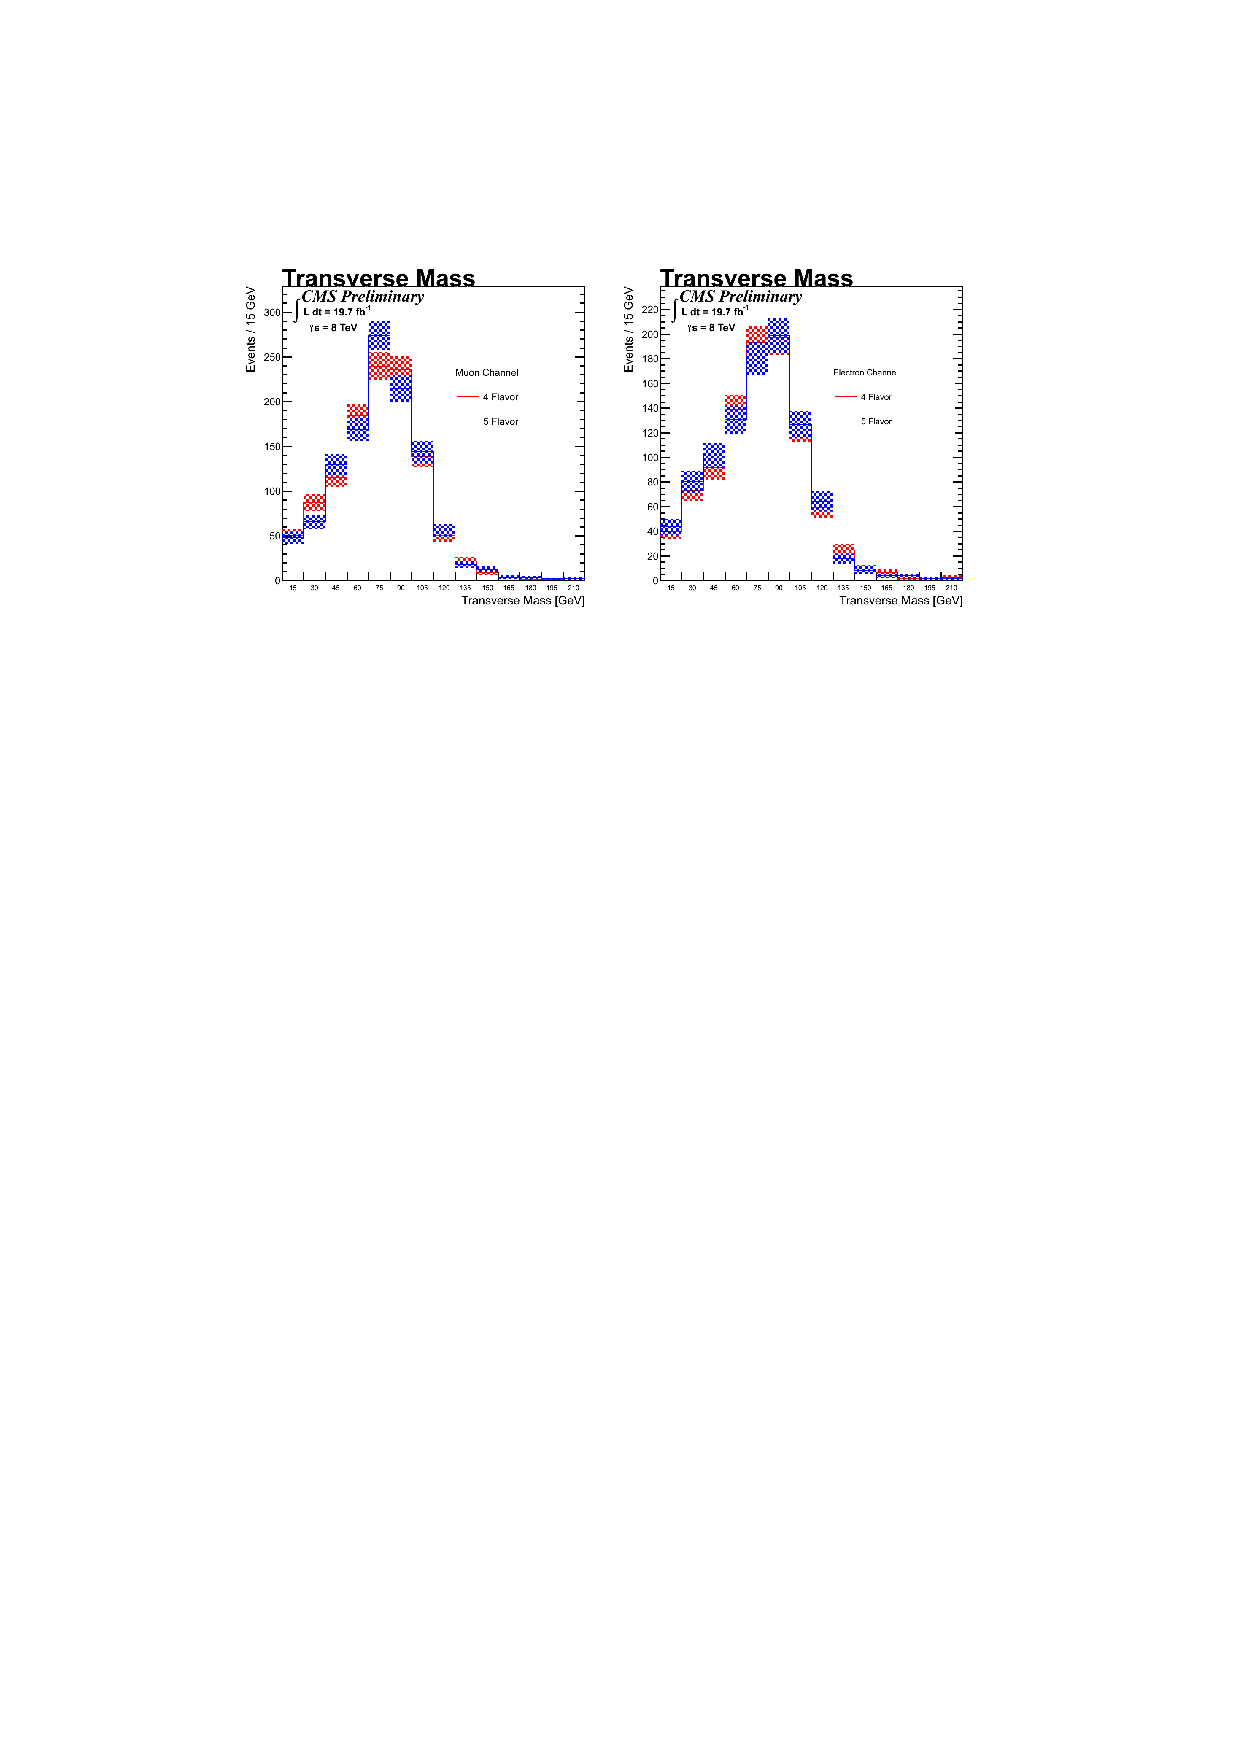
\includegraphics[width=\textwidth]{Figures/4fsvs5fs.pdf}
	\caption[Comparison of the two W+bb samples used to obtain the number of signal events.]{Shape comparison of the two samples used to obtain the number of signal events. The left figure shows the muon channel while the right figure shows the electron channel.}
	\label{fig:4fsvs5fs}
\end{figure}

Signal yields and background yields are extracted using a binned maximum likelihood fit. The details of the fitting procedure are described in \cite{ATL-PHYS-PUB-2011-011}. Due to the observed difference in the overall normalization of the $t\bar{t}$ sample, a simultaneous fit was performed in the Wbb region and in the $t\bar{t}$ multijet control region. 
%The result of the fit is represented as \textit{signal strength} $\mu$ which is the ratio between the cross section under test and the theoretical cross section, in this case Wbb cross-section. 
The predictions for both, signal and background yields, depend on various uncertainties, which are included in the fit as nuisance parameters. The likelihood function is constructed as:
\begin{equation}
\mathcal{L}(\mathrm{data}|\mu,\theta) = Poisson(\mathrm{data}|\mu \cdot s(\theta)+b(\theta))\cdot p(\widetilde{\theta} | \theta).
\end{equation} 
In this expression "data" represents the actual measurements, $\theta$ is a set of nuisance parameters describing the uncertainties while $s(\theta)$ and $b(\theta)$ describe signal and background yields respectively, which depend on the nuisance parameters. $\mu$ is the signal strength, which is the ratio between the cross section under test and the theoretical cross section. $Poisson$ in the context of the binned maximum likelihood represents the product of Poisson probabilities to find $n_i$ events in bin $i$ where the expected number of events is $\mu s_i+b_i$:
\begin{equation}
\prod\limits_{i} \frac{(\mu s_i+b_i)^{n_i}}{n_i!}e^{-(\mu s_i+b_i)}
\end{equation}

Probability density functions $p(\theta)$, with some $\widetilde{\theta}$ as the best estimate of the parameter set describing each of the nuisances, are used to characterize the nuisances. Different options for $pdf$ include flat distribution, Gaussian, log-normal and gamma distribution. In this analysis, systematic uncertainties are treated in two different ways. In cases where the systematic uncertainty does not change the shape of the fitted distribution, a log-normal $pdf$ is used because it is suitable for the description of the positively defined variables like cross-section, luminosity or cut efficiency. Here the value of $\widetilde{\theta}$ in the case of the normalizations of different background shapes corresponds to the normalization of the distribution used in the fit. The width of the log-normal distribution $\rho(\theta)$ is defined by the parameter $\kappa$:
\begin{equation}
\rho(\theta) = \frac{1}{\sqrt{2\pi}ln(\kappa)}exp\left(\frac{(ln(\theta/\widetilde{\theta}))^2}{2(ln \kappa)^2}\right)\frac{1}{\theta}.
\end{equation}
The value of $\kappa$ implies by how much an observable can be larger or smaller, both deviations having a chance of 16$\%$. Another way of treating systematic uncertainties is by producing two additional input shapes for each process affected by some uncertainty, by shifting up and down that parameter by one standard deviation. 
When building the likelihood, each shape uncertainty is associated to a nuisance parameter taken from a unit Gaussian distribution, which is used to interpolate or extrapolate using the specified histograms. After the construction of the likelihood function, parameters $\theta$ and $\mu$ are extracted by minimizing the likelihood function. The next section lists the major sources of systematic uncertainties together with the strategy used for determination of the corresponding nuisance $pdf$.                                                                                                                                                                                                                                                                                                                                                                                                                                                                                                                                                                                                                                                                                                                                                                                                                                                                                                                                                                                                                                                                                                                                                                                                                                                                                                                                                                                                                                                                                                                                                                                                                                                                                                                                                                                                                                                                                                                                                                                                                                                                                                                                                                                                                                                                                                                                                        

%----------------------------------------------------------------------------------------
%	SECTION 2
%----------------------------------------------------------------------------------------

\section{Systematic uncertainties}
\label{sec:syst}

Systematic uncertainties on the expected signal and background yields and shapes affect
the final results. For several systematic variations, a new set of signal and background shapes was created, which may differ both in shape and normalization from the original shape. 
In cases where systematic uncertainty does not change the shape of the distribution used in the fit, only the systematic effect on the normalization was taken into account as described in the previous section. Several sources of systematic variations have been considered:
\subsubsection*{Jet energy scale uncertainty}
		The source of jet energy scale uncertainty arises from the uncertainty on different jet energy corrections applied to unify the detector response in energy and pseudorapidity as described in section \ref{sec:jetCorr}. The uncertainty for each level of corrections is estimated separately and added in quadrature to get the final uncertainty \cite{Chatrchyan:2011ds}. The jet energy scale for each jet is varied within one standard deviation of the applied jet energy corrections and the efficiency of the analysis selection is recomputed to assess the systematic variation on the normalization and shape of the signal and all background components.
\subsubsection*{Jet energy resolution}
        The jet energy resolution in simulation is smeared in order to take into account differences between data and Monte Carlo. The uncertainty on the applied smearing factors is used to produce modified signal and background shapes.  These modified shapes are then used in the final fit.
\subsubsection*{Jet b-tagging efficiencies}
        Jet b-tagging efficiencies are determined for the jets selected in the analysis as described in section \ref{sec:btag}. These efficiencies are applied as weight factors for each event and depend on $p_T$, $\eta$ and flavour of the selected jets. To estimate the effect of the uncertainties on the efficiency determination, each scale factor is shifted up and down by the corresponding uncertainty, and event weights are recalculated. The procedure is done separately for b jet efficiencies and for light flavour mistag rate. The uncertainty for jets from c quark is taken to be twice as large as the one from b jets since there is no proper measurement for this uncertainty. The scale factor variation is found to be of the order of a few percent. 
\subsubsection*{Lepton scale factors}
        Muon and electron trigger, reconstruction, and identification efficiencies are determined in data using the standard tag-and-probe technique with Z bosons as described in \ref{sec:lepEff}. The effects of the corresponding uncertainties were assessed by varying the corresponding scale factors by one standard deviation and producing the modified signal and background shapes. 
\subsubsection*{Lepton energy scale} 
		The lepton energy scale measurement uncertainty corresponds to $1\%$ for muons in the whole detector and electrons in the barrel region. Systematic uncertainty of 2.5$\%$ is associated to the electrons in the endcap region. The effect on the yield is evaluated by varying the lepton energy scale for each lepton within one standard deviation and creating corresponding transverse mass distributions used in the final fit.
\subsubsection*{Unclustered missing energy}
        The uncertainty on missing energy measurement from unclustered energy, e.g. jets with $p_T<$10 GeV and $|\eta|<$4.7 is estimated. The energy scale of such jets is varied by 10$\%$, which is propagated into the calculation of missing energy. New transverse mass distributions are created and taken into account in the final fit.
\subsubsection*{MC samples normalizations}
        The finite size of the signal and background MC samples are included in the normalization uncertainties. Normalizations for each of the Monte-Carlo samples are also allowed to vary within the uncertainties of measured standard model cross-sections. Cross section uncertainties are summarized in the table \ref{tab:SMunc}
\subsubsection*{Luminosity uncertainty}
        Luminosity measurement is performed using cluster counting in the Pixel detector described in section \ref{sec:lumi}. An uncertainty of 2.6$\%$ for the luminosity measurement during 2012 data taking is reported by the CMS luminosity group \cite{CMS-PAS-LUM-13-001}.

\begin{table}[!htb]
\begin{center}
   \begin{tabular} {r c} \hline \hline
        Process         & Cross section uncertainty \\
        \hline
        W+c(c)          & 8.1$\%$ \\
        W+udsg          & 13.2$\%$ \\
        Z+jets          & 7.9$\%$ \\
        Single Top      & 5.4$\%$ \\
        t$\bar{t}$      & 7.4$\%$ \\
        VV              & 8.1$\%$ \\
        \hline\hline
   \end{tabular}
\caption{Standard model cross section uncertainties used in the evaluation of MC normalization systematic effect.}
\label{tab:SMunc}
\end{center}
\end{table}

In figure \ref{fig:shapeVar} the effect of different systematic uncertainties on the shape of the transverse mass distribution is shown for signal and $t\bar{t}$ control region. The shown $M_T$ distributions are obtained by summing signal and all background contributions. The largest systematic variations come from the b-tagging uncertainties. A more detailed study of the final signal strength dependence on the systematic variations is shown in section \ref{sec:systEff}.

\begin{figure}[htbp]
	\centering
		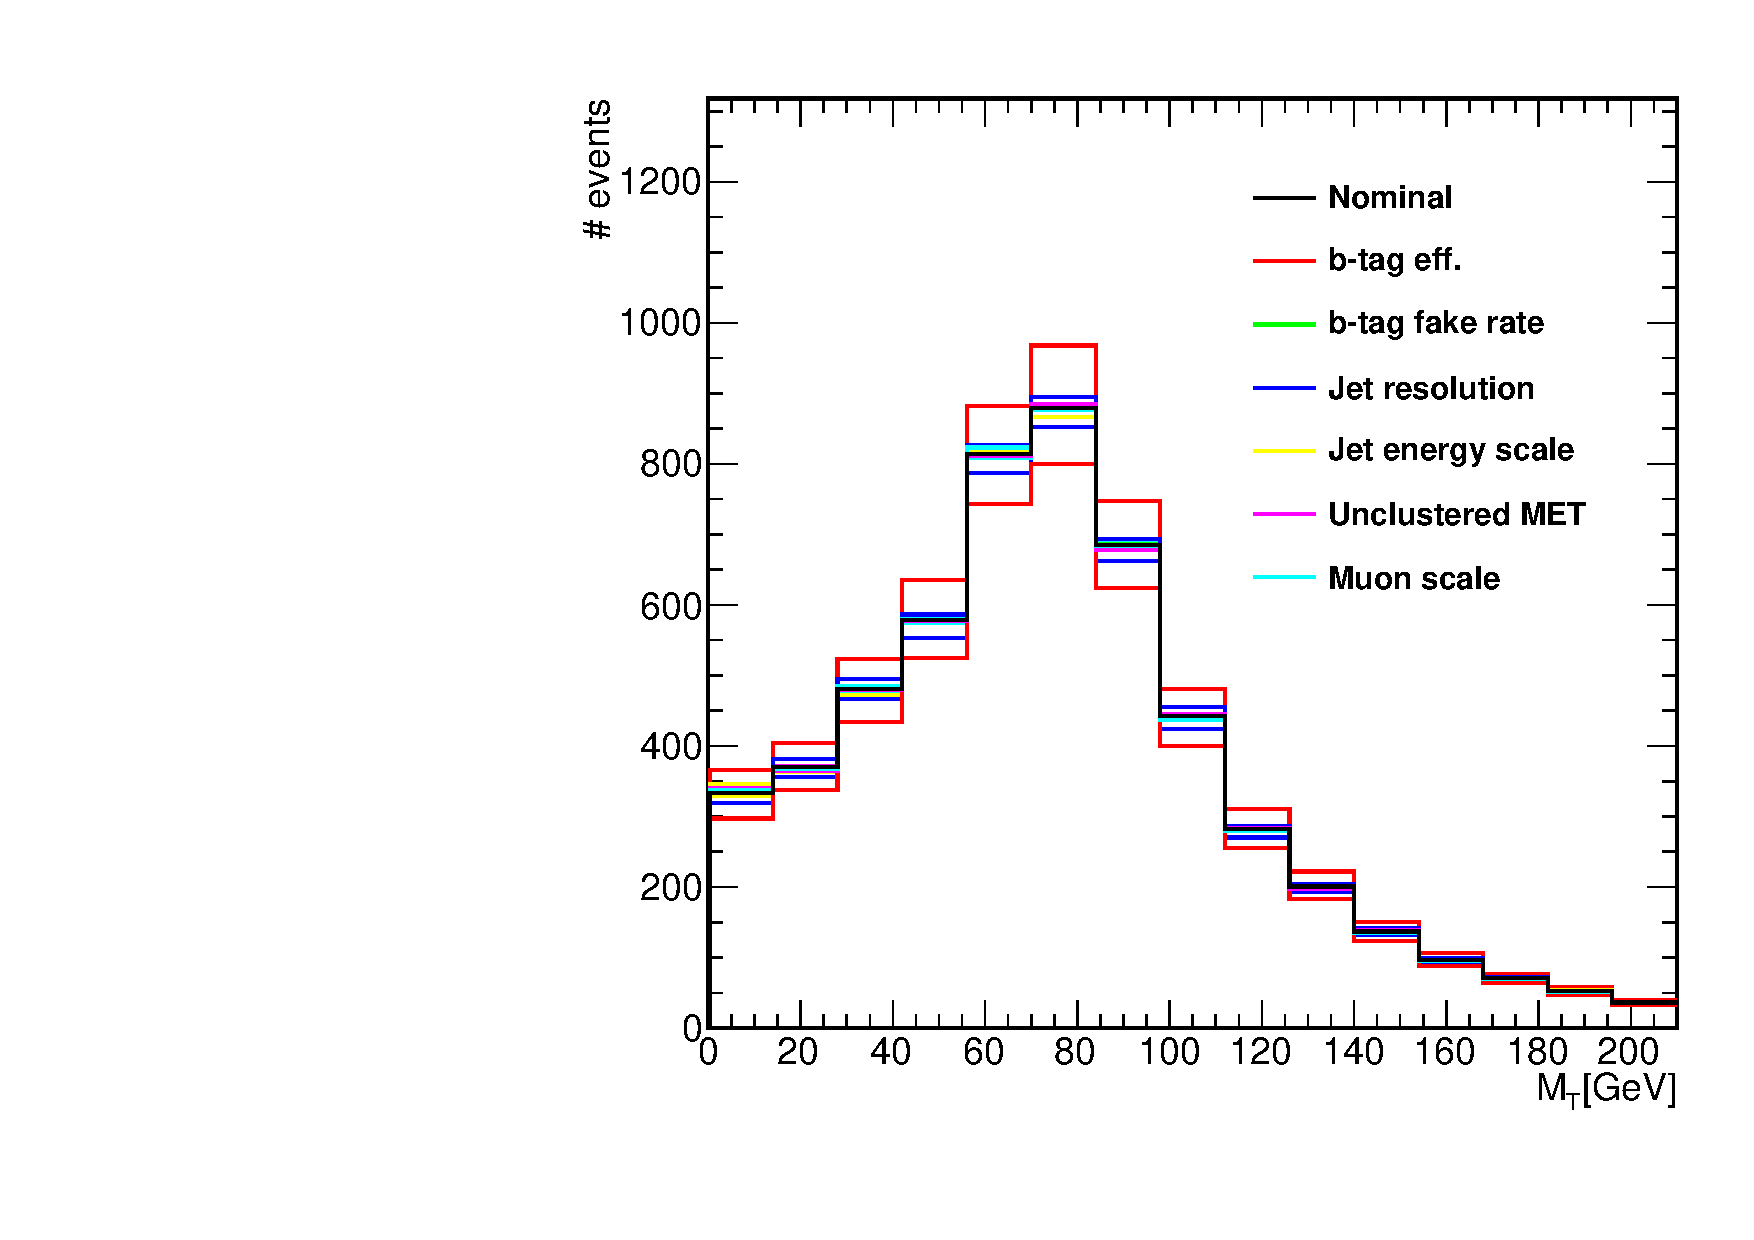
\includegraphics[width=0.49\textwidth]{Figures/syst_Wbb_var.pdf}
		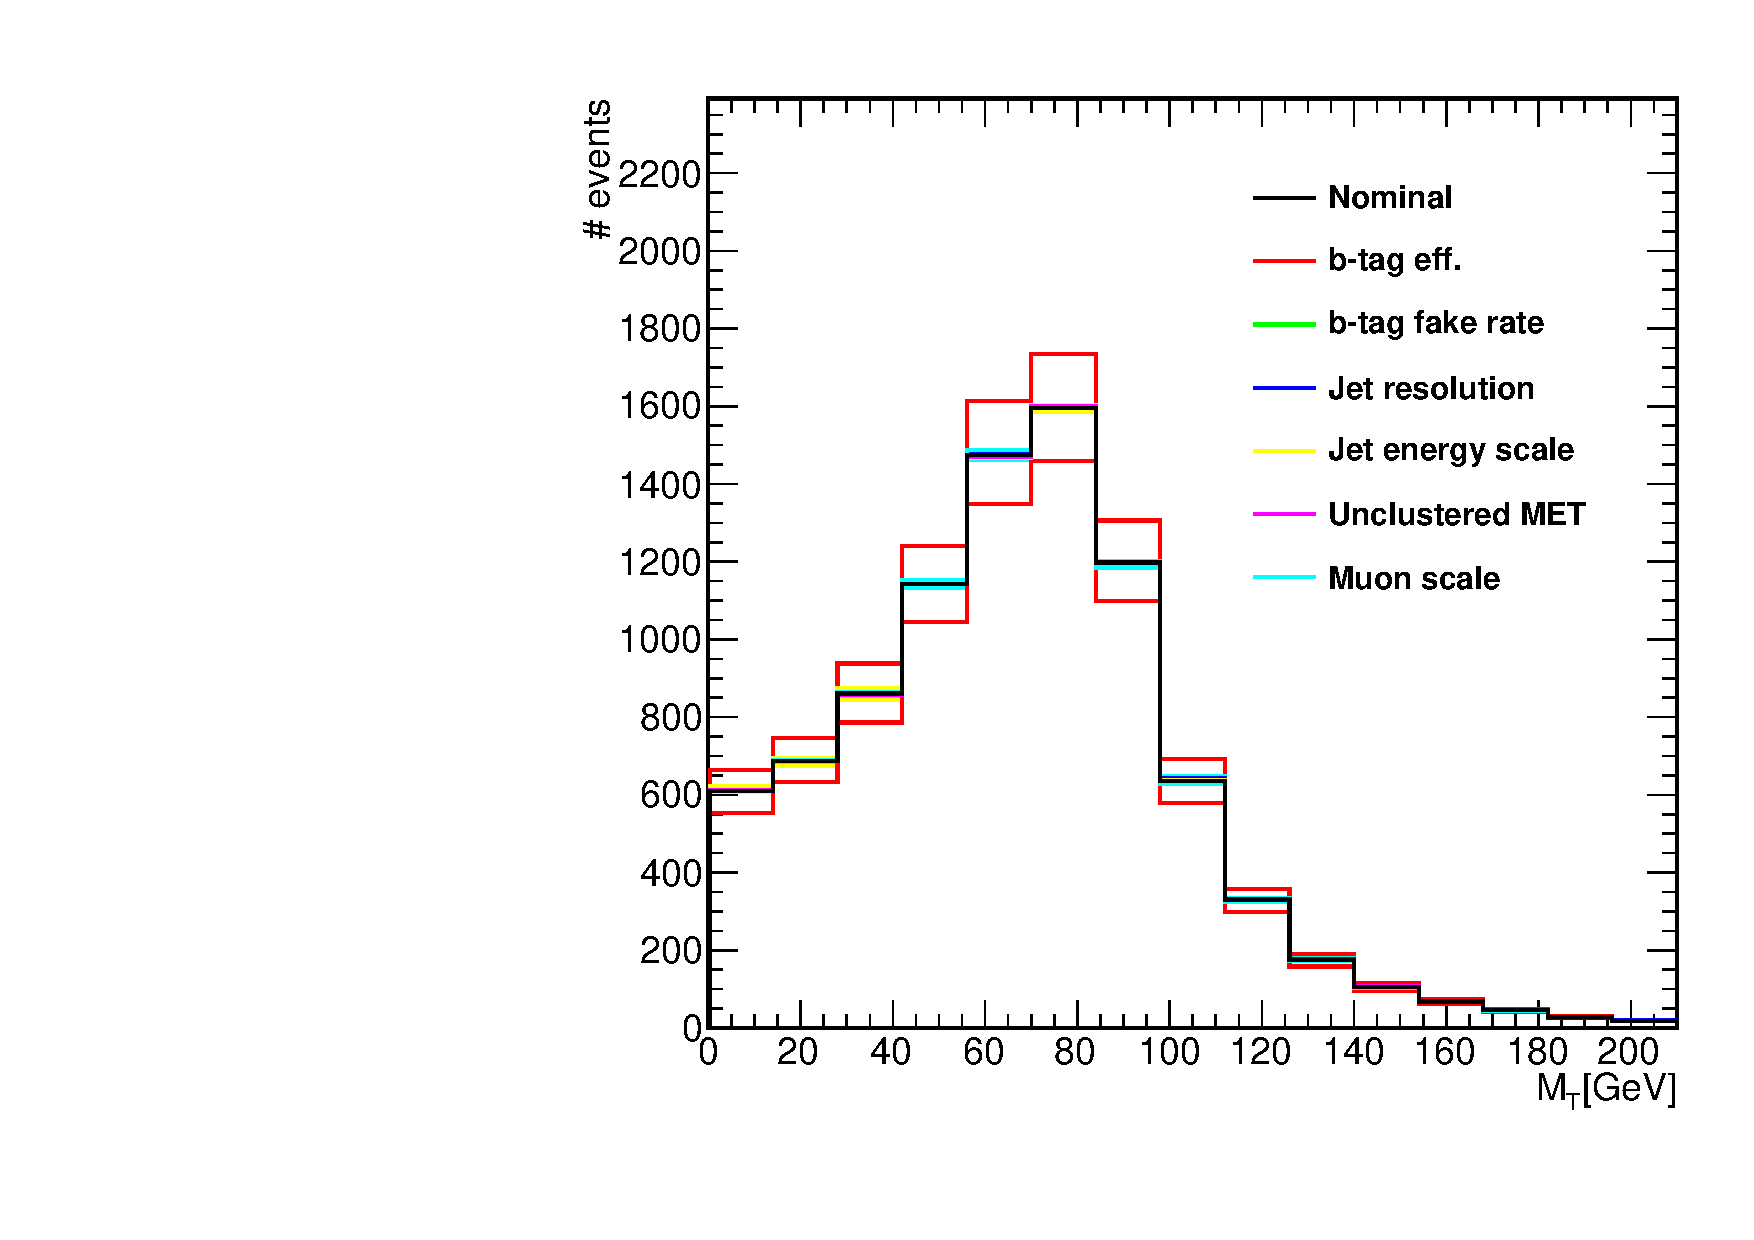
\includegraphics[width=0.49\textwidth]{Figures/syst_TT_var.pdf}
	\caption[Shape of the transverse mass distribution for each systematic variation in both, signal region and $t\bar{t}$ control region.]{Shape of the transverse mass distribution in the muon channel for each systematic variation in both, signal region (\textit{left}) and $t\bar{t}$ control region (\textit{right}).}
	\label{fig:shapeVar}
\end{figure}

%----------------------------------------------------------------------------------------
%	SECTION 3
%----------------------------------------------------------------------------------------
\section{Acceptance and efficiency}
\label{sec:AE}
    
Due to the limitations of the detector, not all produced signal events will be detected. Some final state particles will end up outside the functional part of the detector. The fraction of the phase space covered with a functional detector for signal final state particles is called \textit{acceptance}. The fiducial region in which the cross section is computed corresponds to one lepton with $p_T>$30 GeV and $|\eta|<$2.1. The four-momentum of the lepton is corrected for final state radiation by summing all the photons four-momenta inside a cone of 0.1 from the lepton and cut is applied on the corrected value. Additionally, exactly two jets with $p_T>$ 25 GeV and $|\eta|<$2.4 are required in the event. Jets are clustered from the list of generated particles not considering neutrinos, using anti$-k_T$ algorithm with a cone size of 0.5. Jets are required to contain at least one particle originating from a B hadron decay within a cone of 0.5 from the jet axis in the list of the clustered particles. Fiducial region requirements are summarized in table \ref{tab:fiducial}.             
\begin{table}[!htb]
\begin{center}
   \begin{tabular} {l c} \hline \hline
        Variable         & Cut \\
        \hline
        Lepton $p_T$    & $>$ 30\ GeV \\
        Lepton $|\eta|$   & $<$ 2.1 \\
        Jet $p_T$       & $>$ 25  \\
        Jet $|\eta|$      & $<$ 2.4 \\
        $\Delta R$(jet, B hadron) & $<$ 0.5 \\
        \hline\hline
   \end{tabular}
\caption{Fiducial cuts used for cross section measurements.}
\label{tab:fiducial}
\end{center}
\end{table}
However, a fraction of the events that fall into the fiducial volume will not be detected due to trigger and reconstruction inefficiencies or selection cuts imposed at trigger or analysis level. Usually, the acceptance and efficiency are estimated as a single quantity, which is a product of these two numbers, defined as:
\begin{equation}
A\times \epsilon=\frac{\mathrm{number\ of\ selected\ Wbb\ events}}{\mathrm{number\ of\ generated\ Wbb\ events\ in\ the\ fiducial\ volume}}
\end{equation}
This ratio is computed using simulated Wbb sample for each of the channels separately. The number of selected events is obtained by applying the selection cuts described in \ref{sec:selection}. The number of generated events is obtained by applying generator-level cuts summarized in table \ref{tab:fiducial}. As this ratio is derived from simulation, it is necessary to correct it for differences between data and Monte-Carlo. These corrections include pile-up  $w^{PU}$, lepton trigger, reconstruction and identification scale factors $w^{lep}$, and b-tagging scale factors $w^{b-tag}$ all described in \ref{sec:mcSF}. With all the corrections, $A\times \epsilon$ for each channel becomes:
\begin{equation}
A\times \epsilon = \frac{\sum^{sel} w^{lep} w^{PU} w^{b-tag}}{N_{fiducial}^{gen}}
\end{equation}
where the sum in the numerator runs over selected events.
Obtained results are summarized in table \ref{tab:AE} for each channel.

\begin{table}[!htb]
\begin{center}
   \begin{tabular} {r c} \hline \hline
        Channel         & A$\times \epsilon$ \\
        \hline
        Muon channel         & 9.14 $\pm$ 0.18 $\%$ \\
        Electron channel     & 7.66 $\pm$ 0.17 $\%$ \\
        \hline\hline
   \end{tabular}
\caption{Results of the A$\times \epsilon$ determination for both, muon and electron channel together with the statistical uncertainty.}
\label{tab:AE}
\end{center}
\end{table}



%----------------------------------------------------------------------------------------
%	SECTION 5
%----------------------------------------------------------------------------------------

\section{Results}
\label{sec:res}

Transverse mass distributions in the signal region and $t\bar{t}$ region were fitted simultaneously in order to obtain the signal strength for Wbb. Yields before and after the fit are shown in Table \ref{tab:yieldsMu} for the muon channel and \ref{tab:yieldsEle} for the electron channel. The obtained signal strength values are:
\begin{align*}
\mu_{muon} &= 1.37 \pm 0.07\mathrm{(stat.)} \pm 0.20 \mathrm{(syst.)}\\\
\mu_{ele} &= 1.67 \pm 0.08\mathrm{(stat.)} \pm 0.27\mathrm{(syst.)}
\end{align*}
The total uncertainty was obtained by including both systematic and statistical uncertainties. Another fit was performed without systematic uncertainties in order to obtain the statistical error. The total systematic error was computed by subtracting in quadrature the statistical error from the total error. 
Figures \ref{fig:Wbb_postfit_mu} and \ref{fig:Wbb_postfit_ele} show the most important detector distribution after performing the fit for the muon and electron channels respectively. The recovered distributions show a good agreement between data and simulation for all considered distributions.

\begin{table}[h!]
\caption{Yields obtained in the muon channel before and after the fitting procedure.}
\label{tab:yieldsMu}

 \begin{adjustbox}{width=\textwidth,center=\textwidth}
   \begin{tabular} {c|cc|cc} \hline\hline
			 Sample & ~~~Prefit yields~~~ & ~~~~Fitted yields~~~ & Prefit yields($M_T>45$GeV) & Fitted yields($M_T>45$GeV) \\ 
 \hline
W+bb&1129.7$\pm$25.5&1629.1$\pm$80.5&871.7$\pm$29.5&1254.5$\pm$75.0\\
W+cc&68.9$\pm$7.4&81.9$\pm$9.8&52.8$\pm$7.3&62.6$\pm$9.1\\
W+udscg&47.1$\pm$10.8&61.4$\pm$15.6&35.8$\pm$6.0&46.8$\pm$14.3\\
Z+jets&208.7$\pm$22.4&217.0$\pm$18.8&121.8$\pm$11.0&126.6$\pm$14.4\\
Single Top&913.1$\pm$16.7&986.4$\pm$33.4&700.2$\pm$26.5&748.1$\pm$30.4\\
T$\bar{T}$&3093.2$\pm$13.0&3488.0$\pm$36.2&2499.6$\pm$50.0&2713.9$\pm$32.8\\
VV&145.2$\pm$3.1&151.8$\pm$6.1&108.4$\pm$10.4&113.1$\pm$5.7\\
QCD&1110.5$\pm$28.2&908.4$\pm$33.6&293.9$\pm$17.1&240.4$\pm$11.6\\
\hline
Sum &6716.3$\pm$50.7&7524.1$\pm$103.8&4684.2$\pm$68.4&5306.0$\pm$91.0\\
\hline
Data&\multicolumn{2}{c}{7481.0}&\multicolumn{2}{c}{5372.0}\\
   \hline\hline
   \end{tabular}
 \end{adjustbox}


\end{table}
\begin{table}[h!]
\caption{Yields obtained in the electron channel before and after the fitting procedure.}
\label{tab:yieldsEle}
 \begin{adjustbox}{width=1.\textwidth,center=\textwidth}
   \begin{tabular} {c|cc|cc} \hline\hline
			 Sample & ~~~Prefit yields~~~ & ~~~~Fitted yields~~~ & Prefit yields($M_T>45$GeV) & Fitted yields($M_T>45$GeV) \\ 
 \hline
W+bb&940.6$\pm$23.3&1533.4$\pm$220.0&715.8$\pm$22.9&1172.7$\pm$170.7\\
W+cc&68.6$\pm$8.2&60.5$\pm$18.4&60.1$\pm$7.3&52.2$\pm$17.2\\
W+udsg&15.4$\pm$5.2&13.6$\pm$8.6&12.5$\pm$8.2&10.9$\pm$6.9\\
Z+jets&201.1$\pm$21.4&176.5$\pm$28.9&88.7$\pm$17.2&93.6$\pm$21.0\\
Single Top&719.6$\pm$14.8&661.4$\pm$62.2&547.6$\pm$14.6&500.8$\pm$49.2\\
T$\bar{T}$&2496.8$\pm$11.6&2315.5$\pm$111.9&2056.3$\pm$11.3&1837.4$\pm$89.4\\
VV&110.2$\pm$2.7&106.5$\pm$10.7&85.4$\pm$2.7&83.9$\pm$8.8\\
QCD&1585.3$\pm$22.5&1696.2$\pm$125.4&787.2$\pm$15.2&838.2$\pm$62.0\\
\hline
Sum &6137.8$\pm$44.3&6563.6$\pm$404.6&4353.6$\pm$39.0&4589.7$\pm$210.4\\
\hline
Data&\multicolumn{2}{c}{6530.0}&\multicolumn{2}{c}{4639.0}\\
   \hline\hline
   \end{tabular}
 \end{adjustbox}

\end{table}

\begin{figure}[htbp]
	\centering
		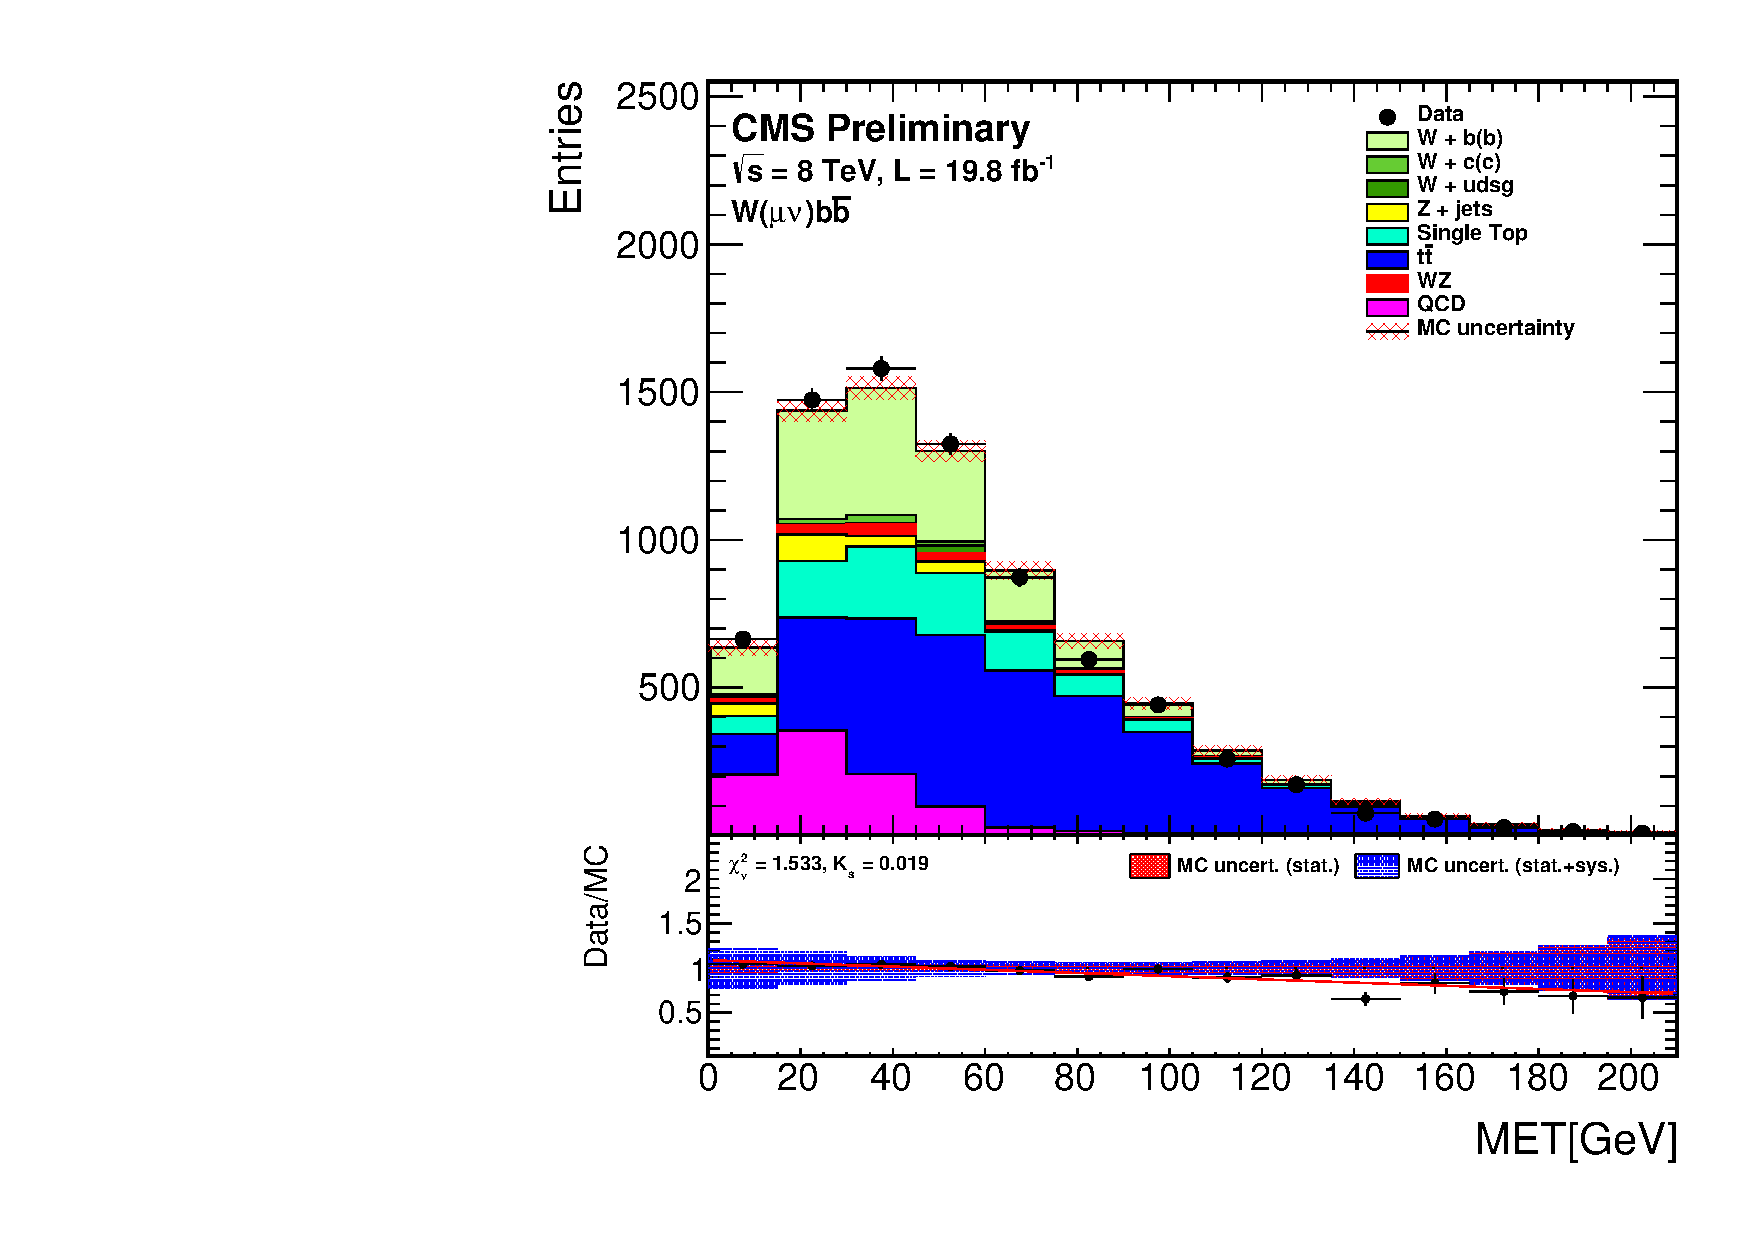
\includegraphics[width=0.48\textwidth]{Figures/Results/Muon/postfit/Wbb_GetMET_doQCD1.pdf}
		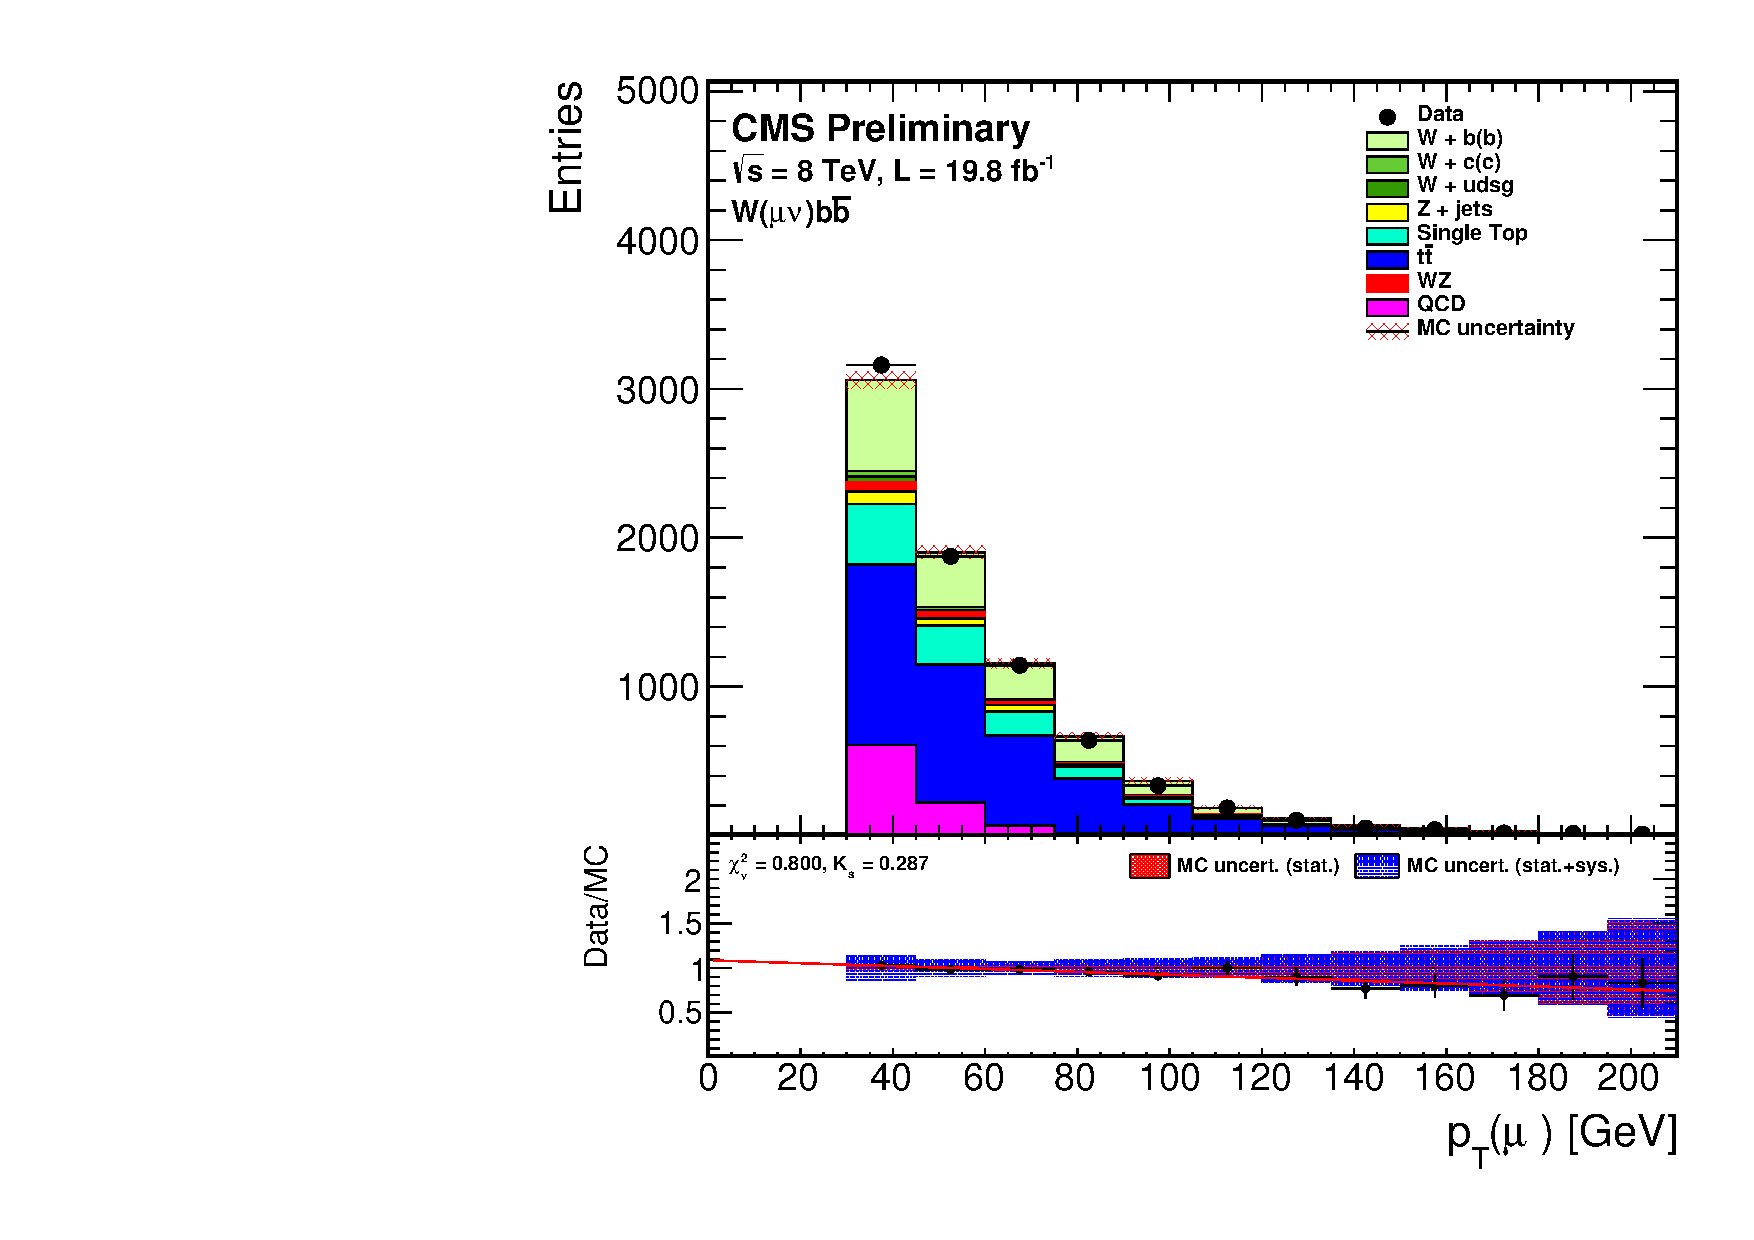
\includegraphics[width=0.48\textwidth]{Figures/Results/Muon/postfit/Wbb_vLepton_pt_doQCD1.pdf}
		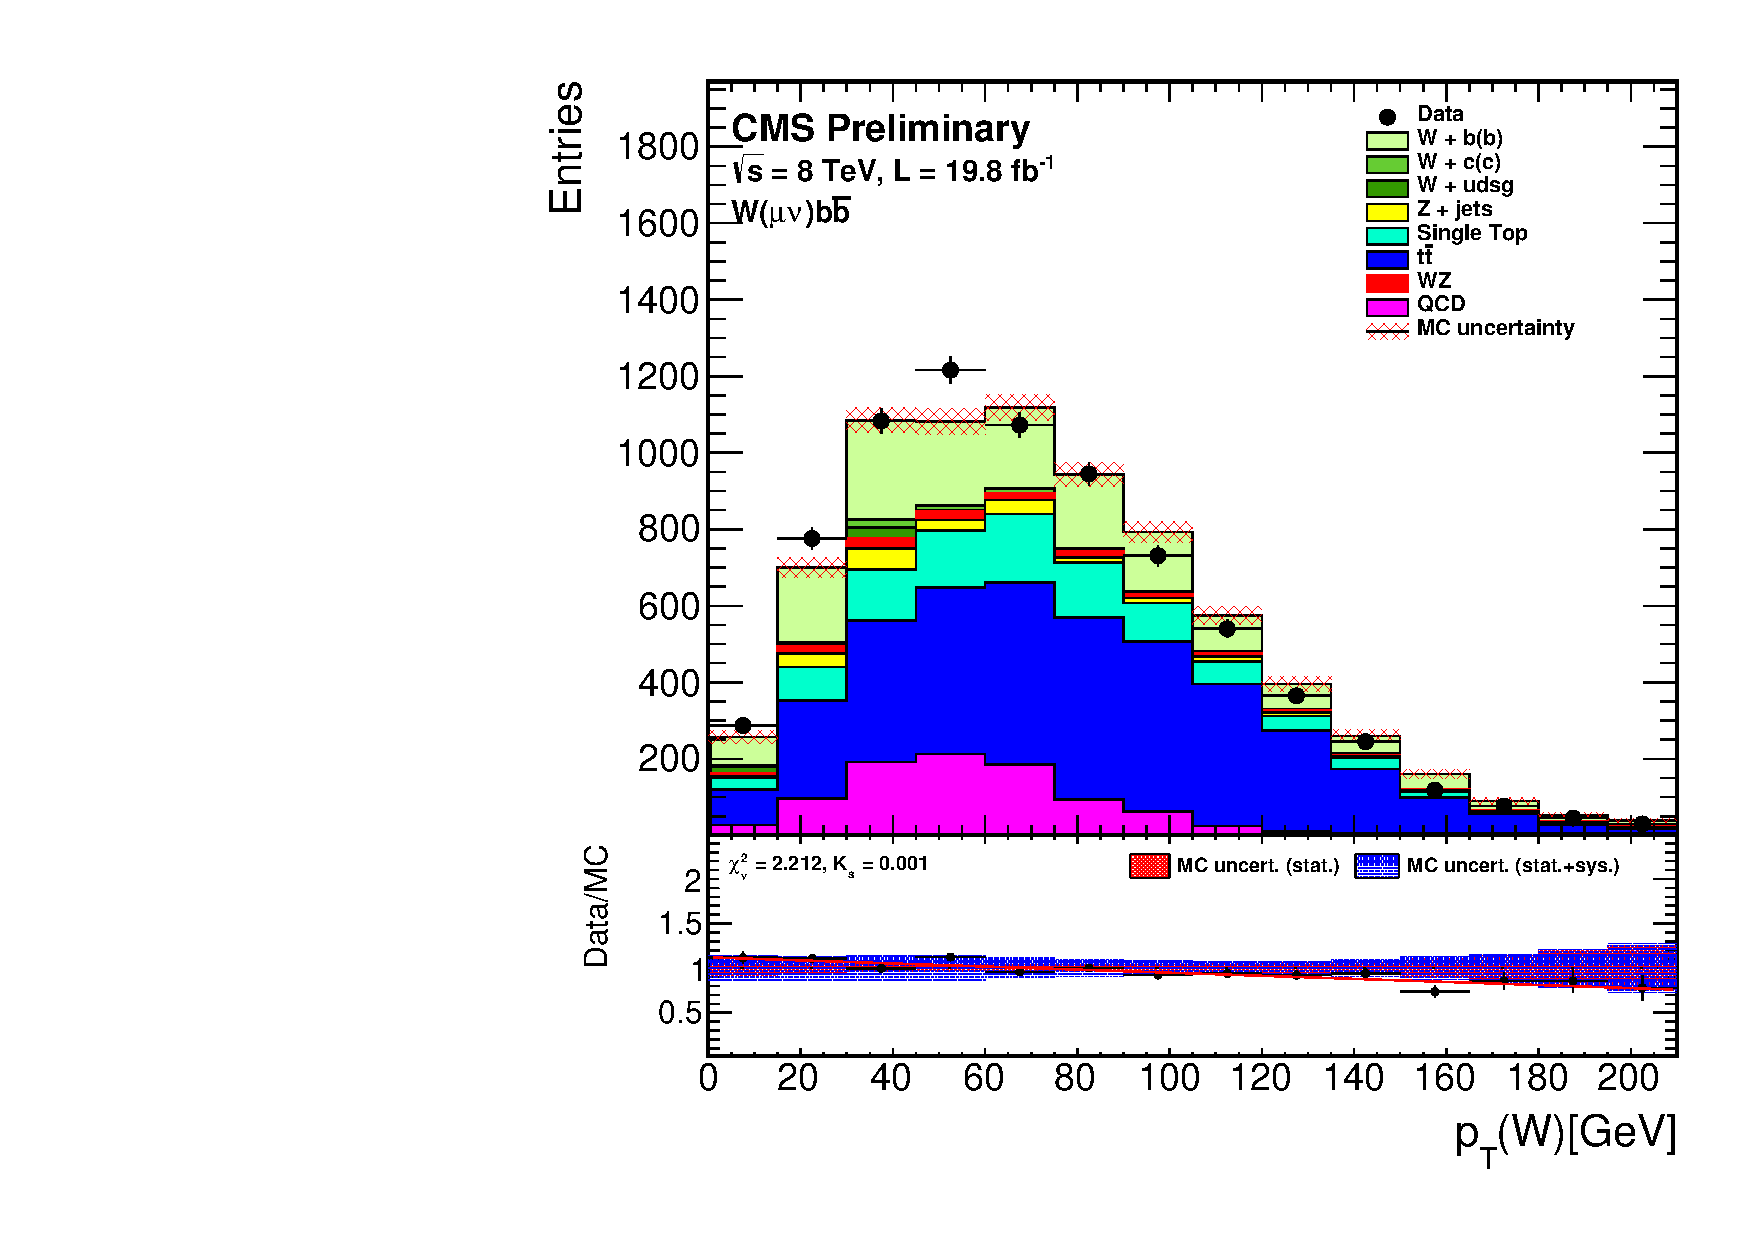
\includegraphics[width=0.48\textwidth]{Figures/Results/Muon/postfit/Wbb_GetWpt_doQCD1.pdf}
		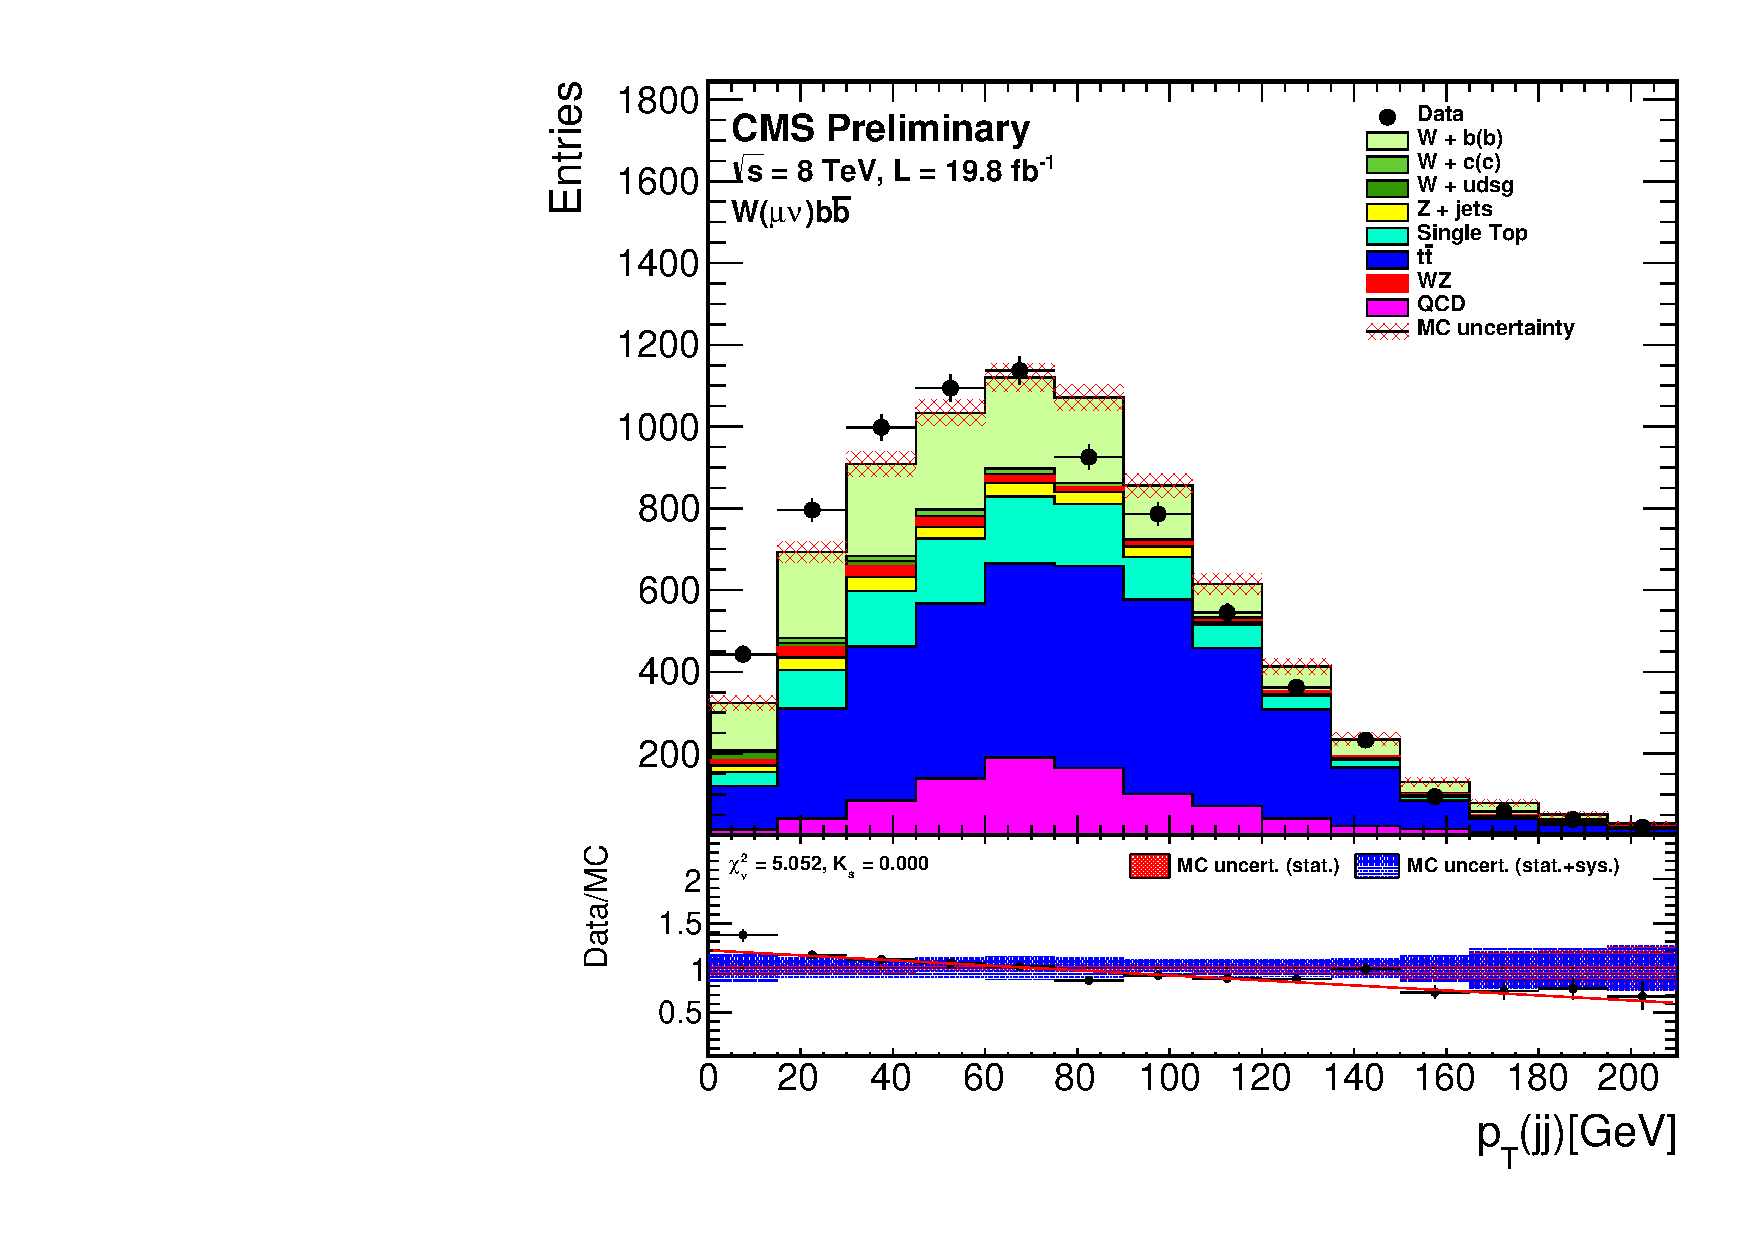
\includegraphics[width=0.48\textwidth]{Figures/Results/Muon/postfit/Wbb_H_pt_doQCD1.pdf}
		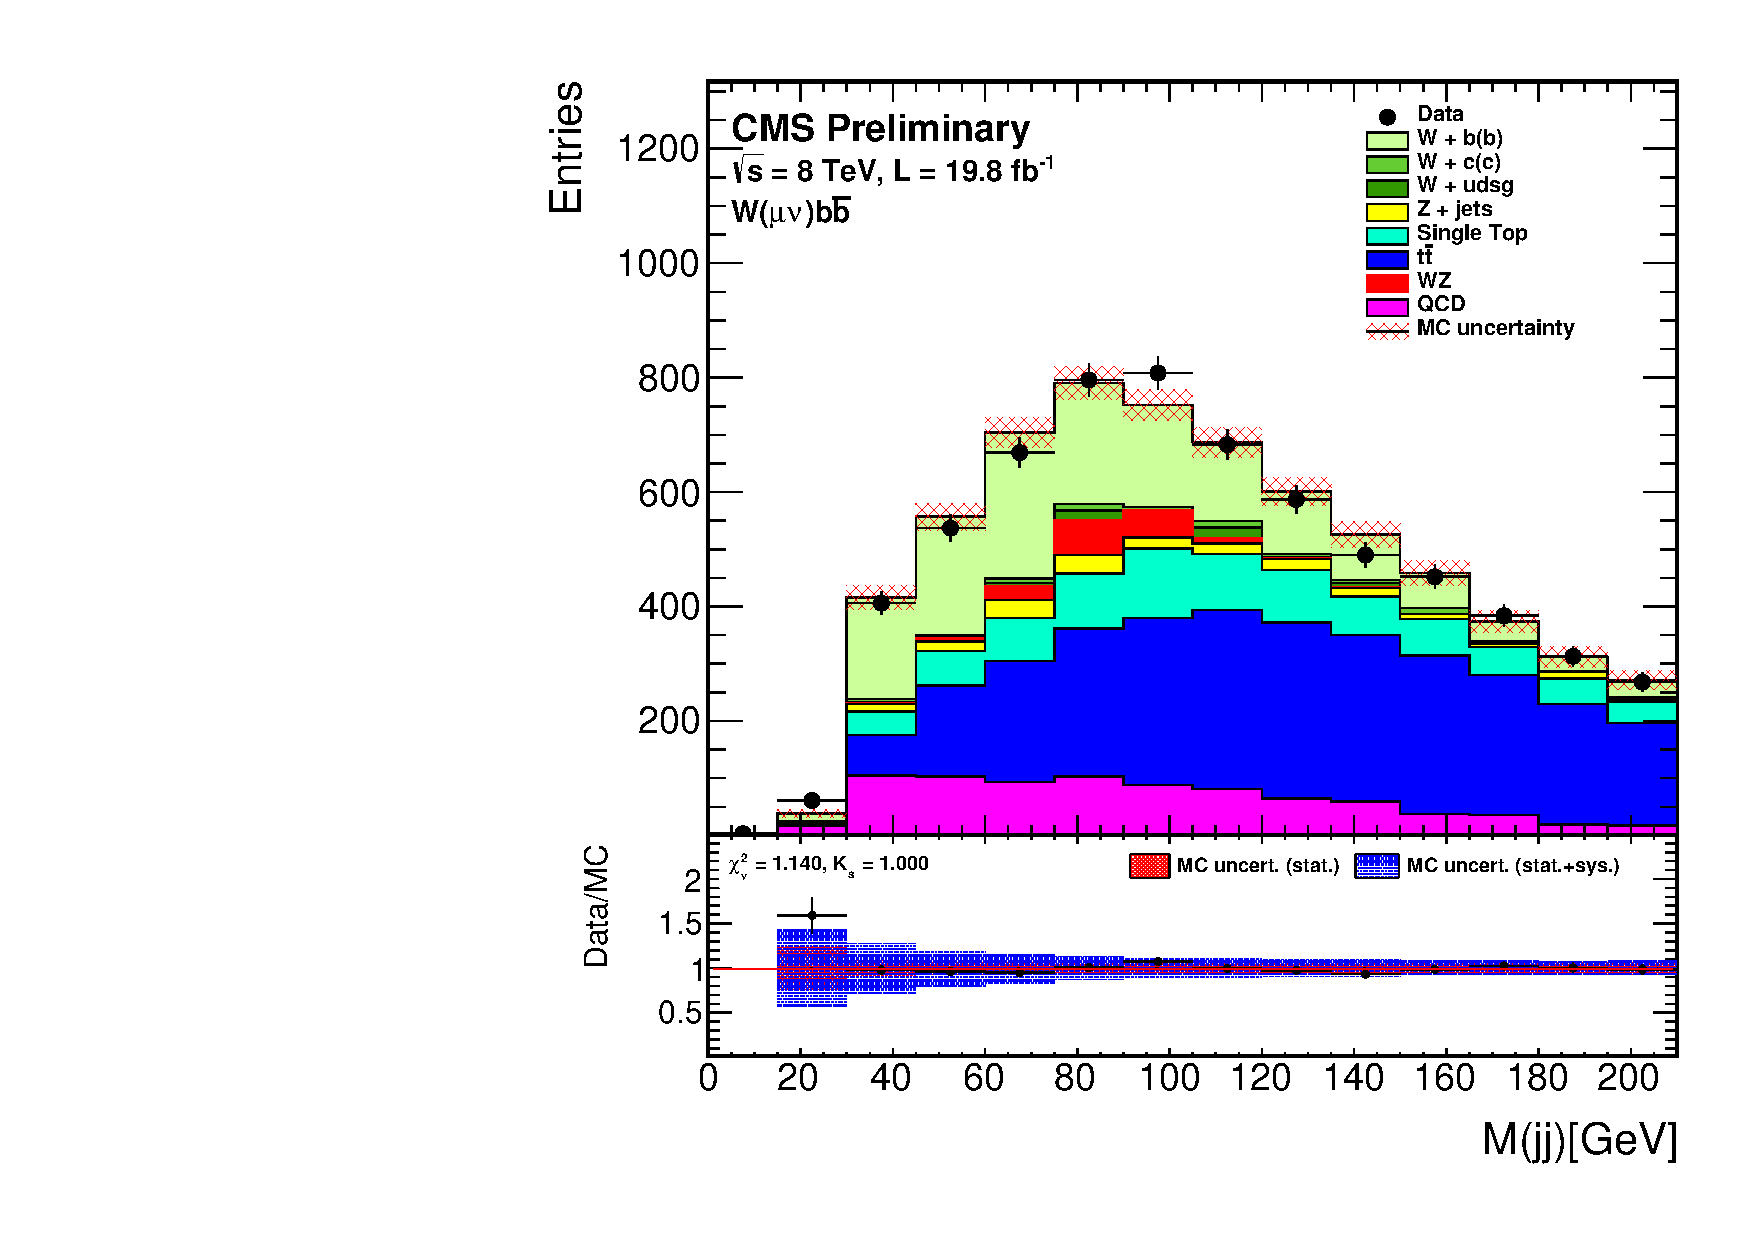
\includegraphics[width=0.48\textwidth]{Figures/Results/Muon/postfit/Wbb_H_mass_doQCD1.pdf}
		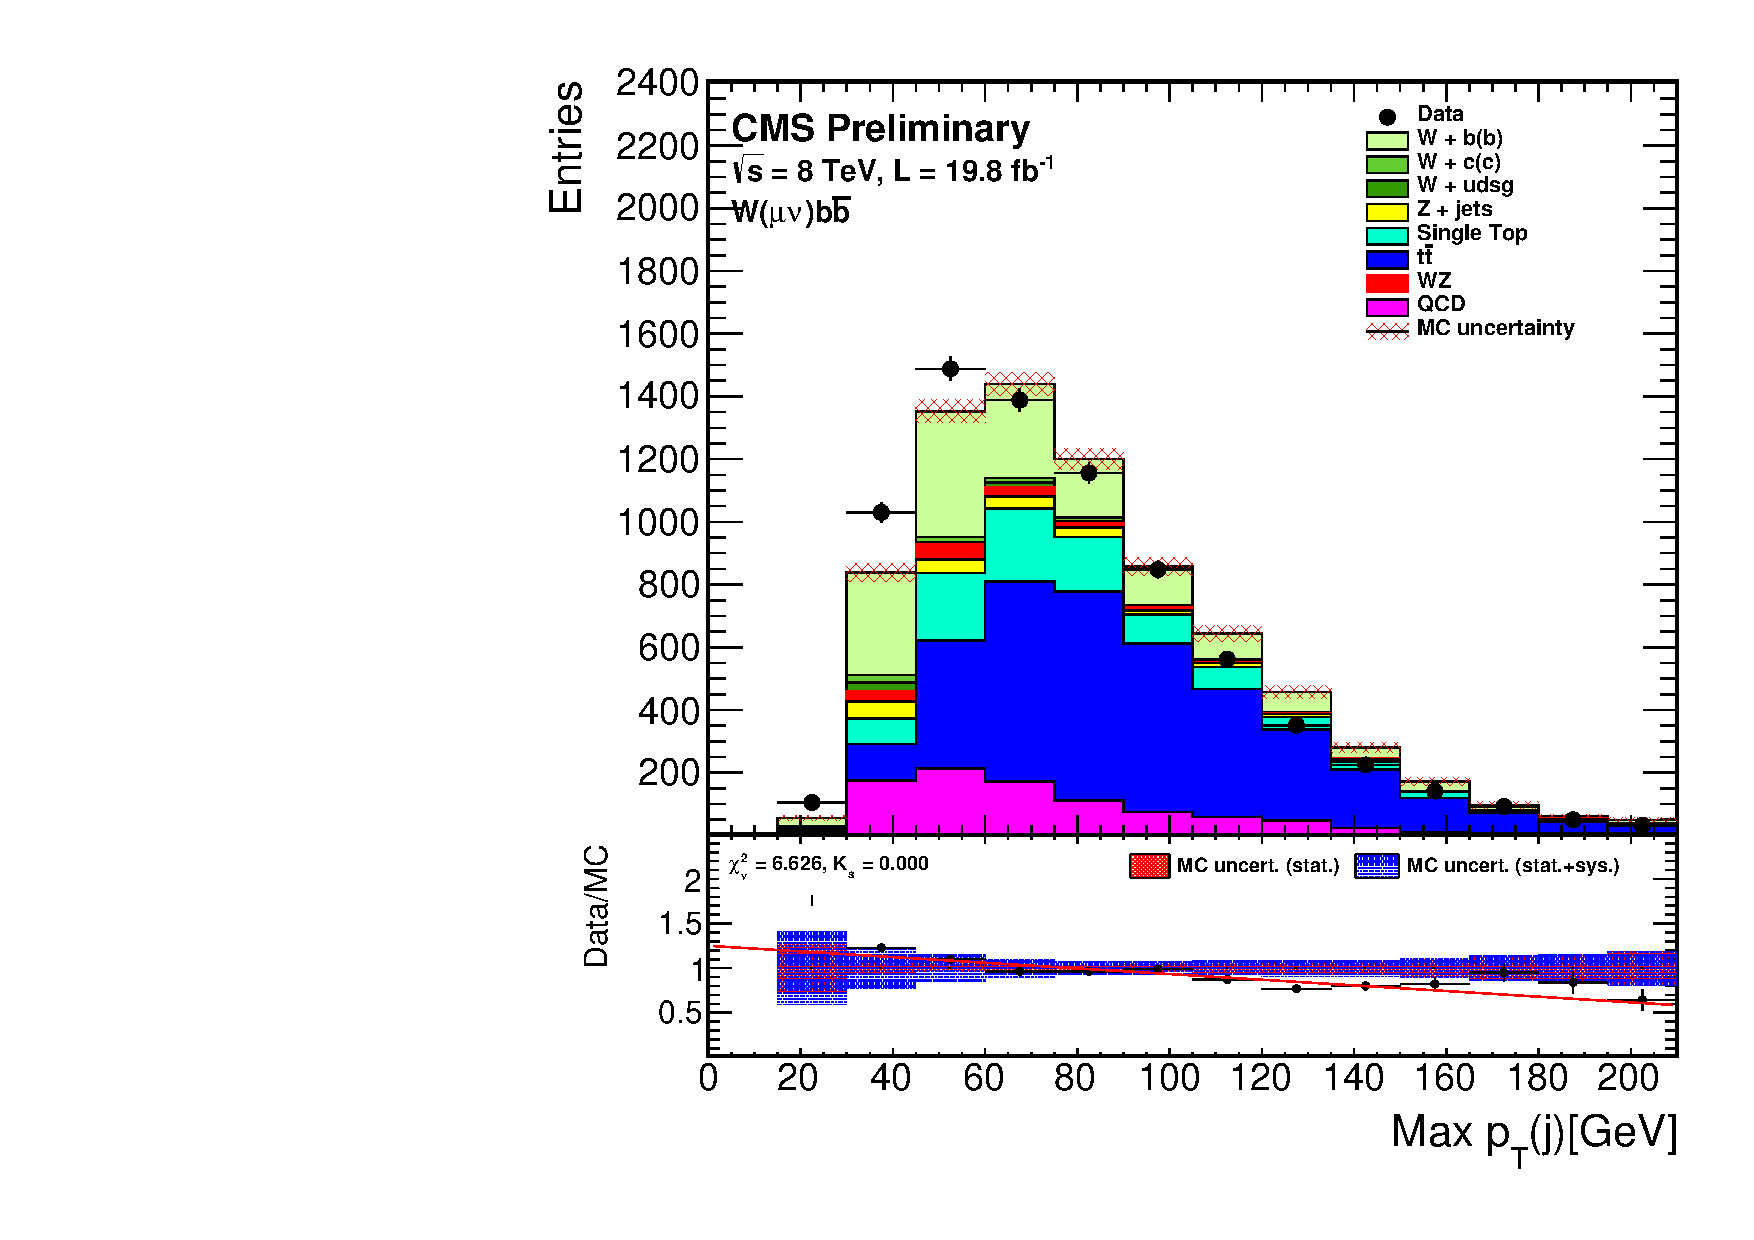
\includegraphics[width=0.48\textwidth]{Figures/Results/Muon/postfit/Wbb_max_hJet_pt_doQCD1.pdf}		
		%\rule{35em}{0.5pt}
	\caption{Muon channel distributions after the fit.}
	\label{fig:Wbb_postfit_mu}
\end{figure}

\begin{figure}[htbp]
	\centering
		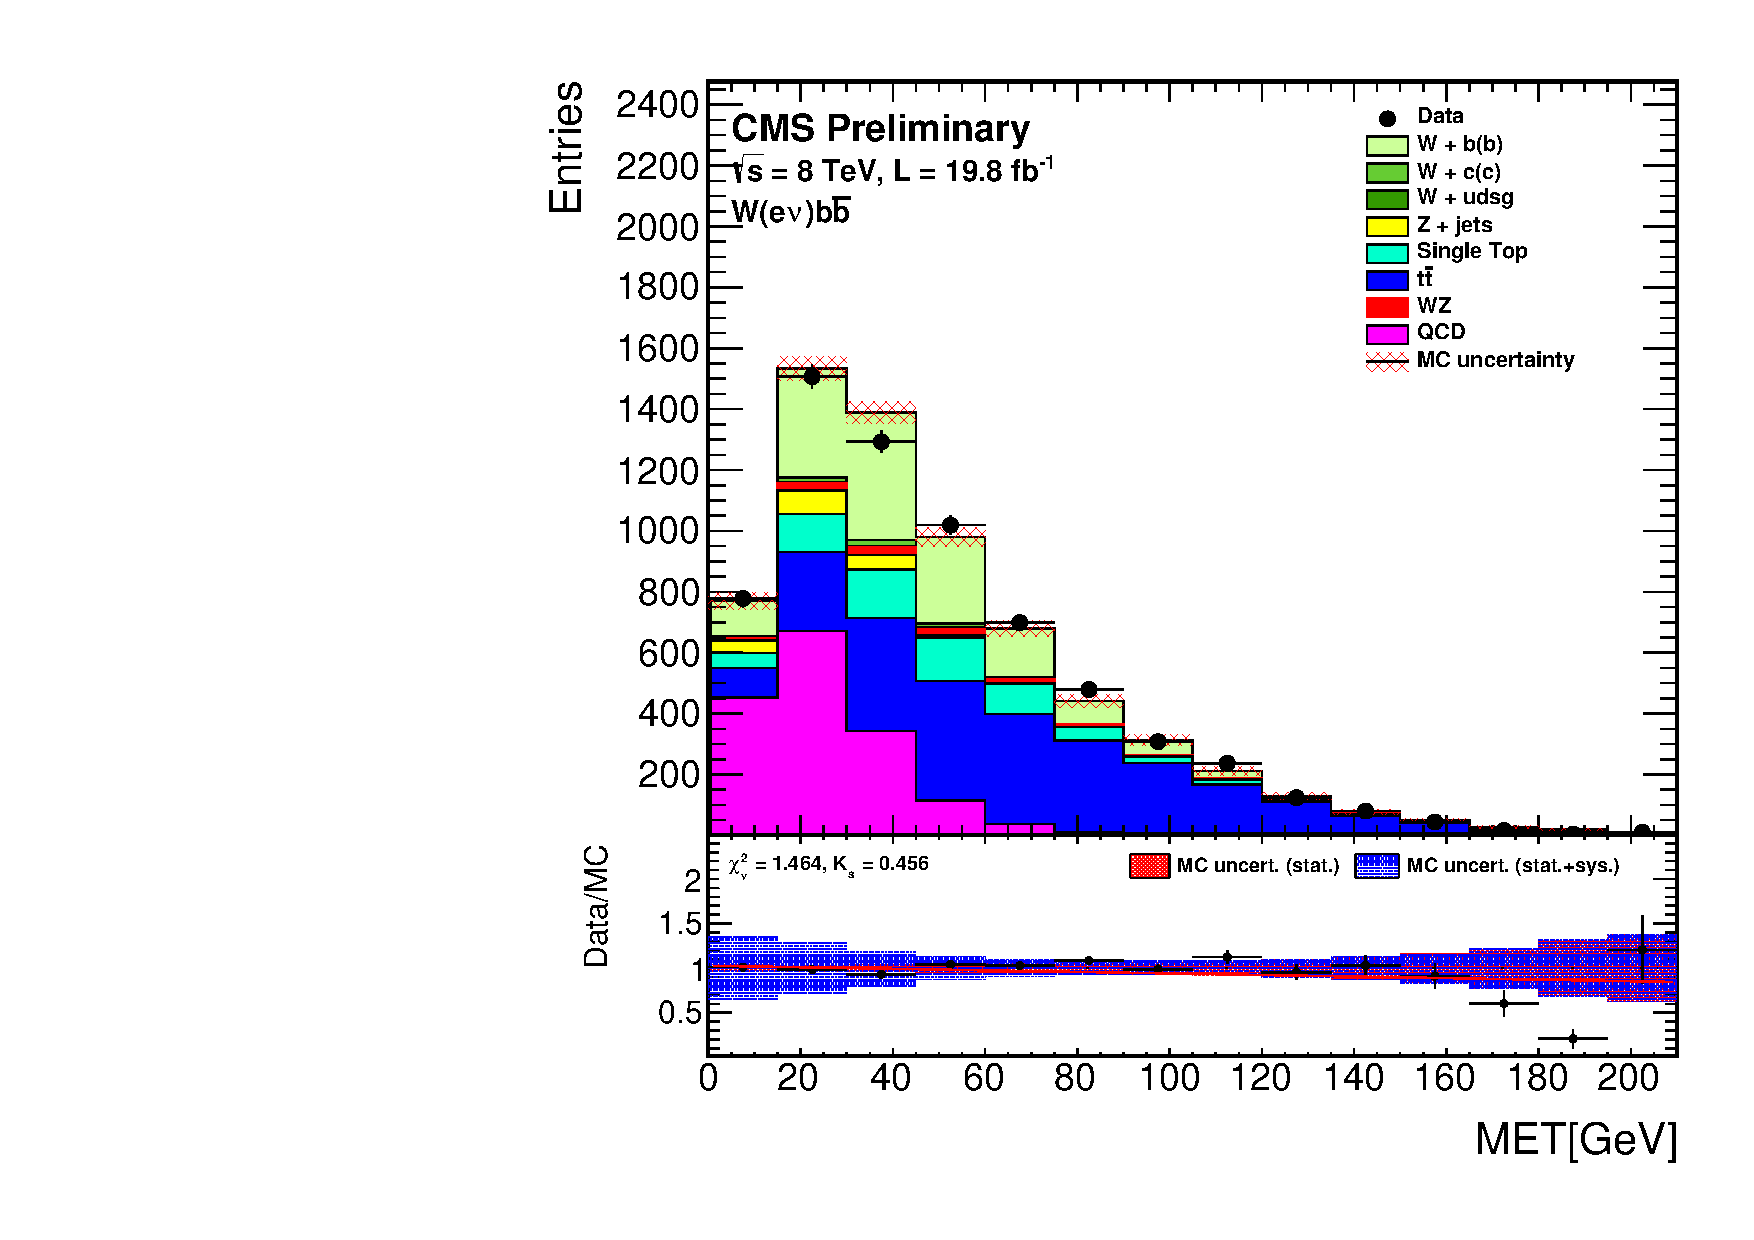
\includegraphics[width=0.48\textwidth]{Figures/Results/Electron/postfit/Wbb_GetMET_doQCD1.pdf}
		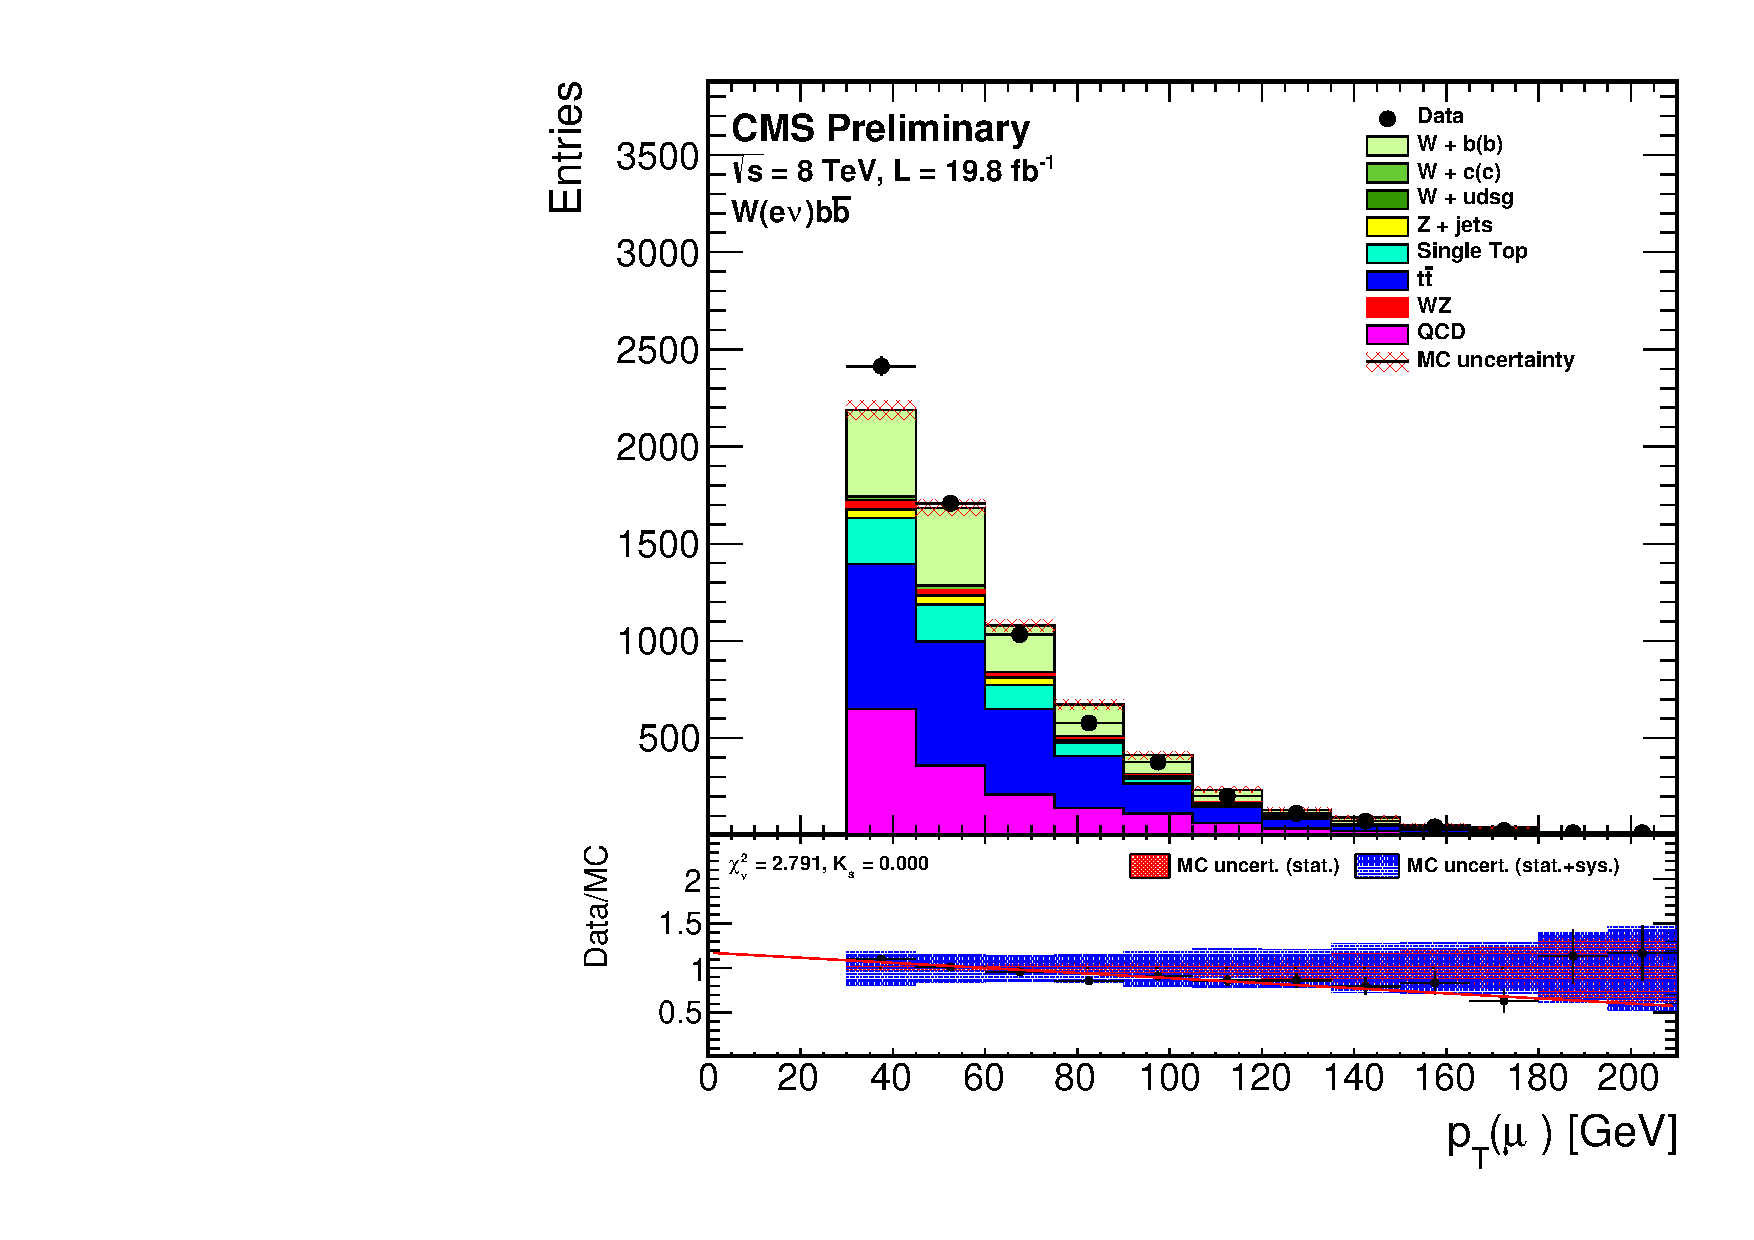
\includegraphics[width=0.48\textwidth]{Figures/Results/Electron/postfit/Wbb_vLepton_pt_doQCD1.pdf}
		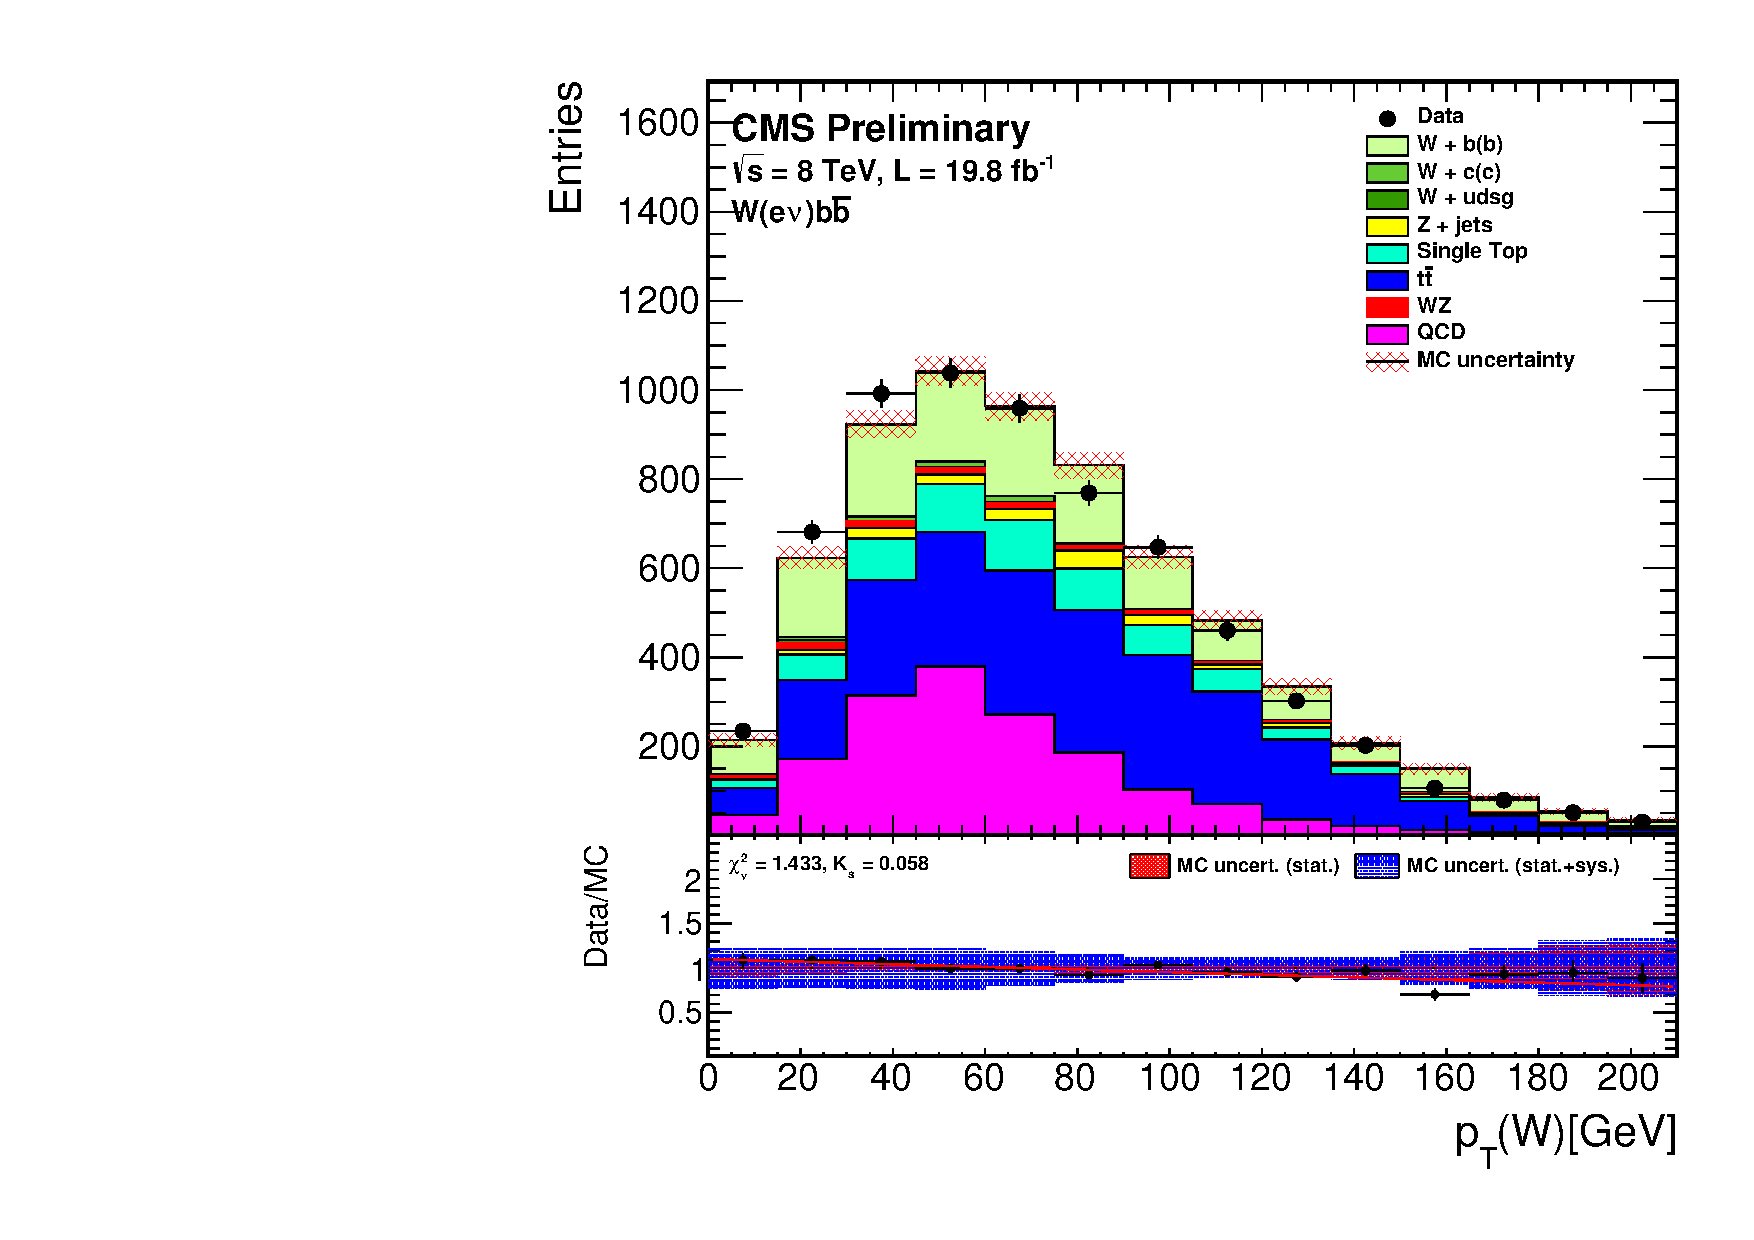
\includegraphics[width=0.48\textwidth]{Figures/Results/Electron/postfit/Wbb_GetWpt_doQCD1.pdf}
		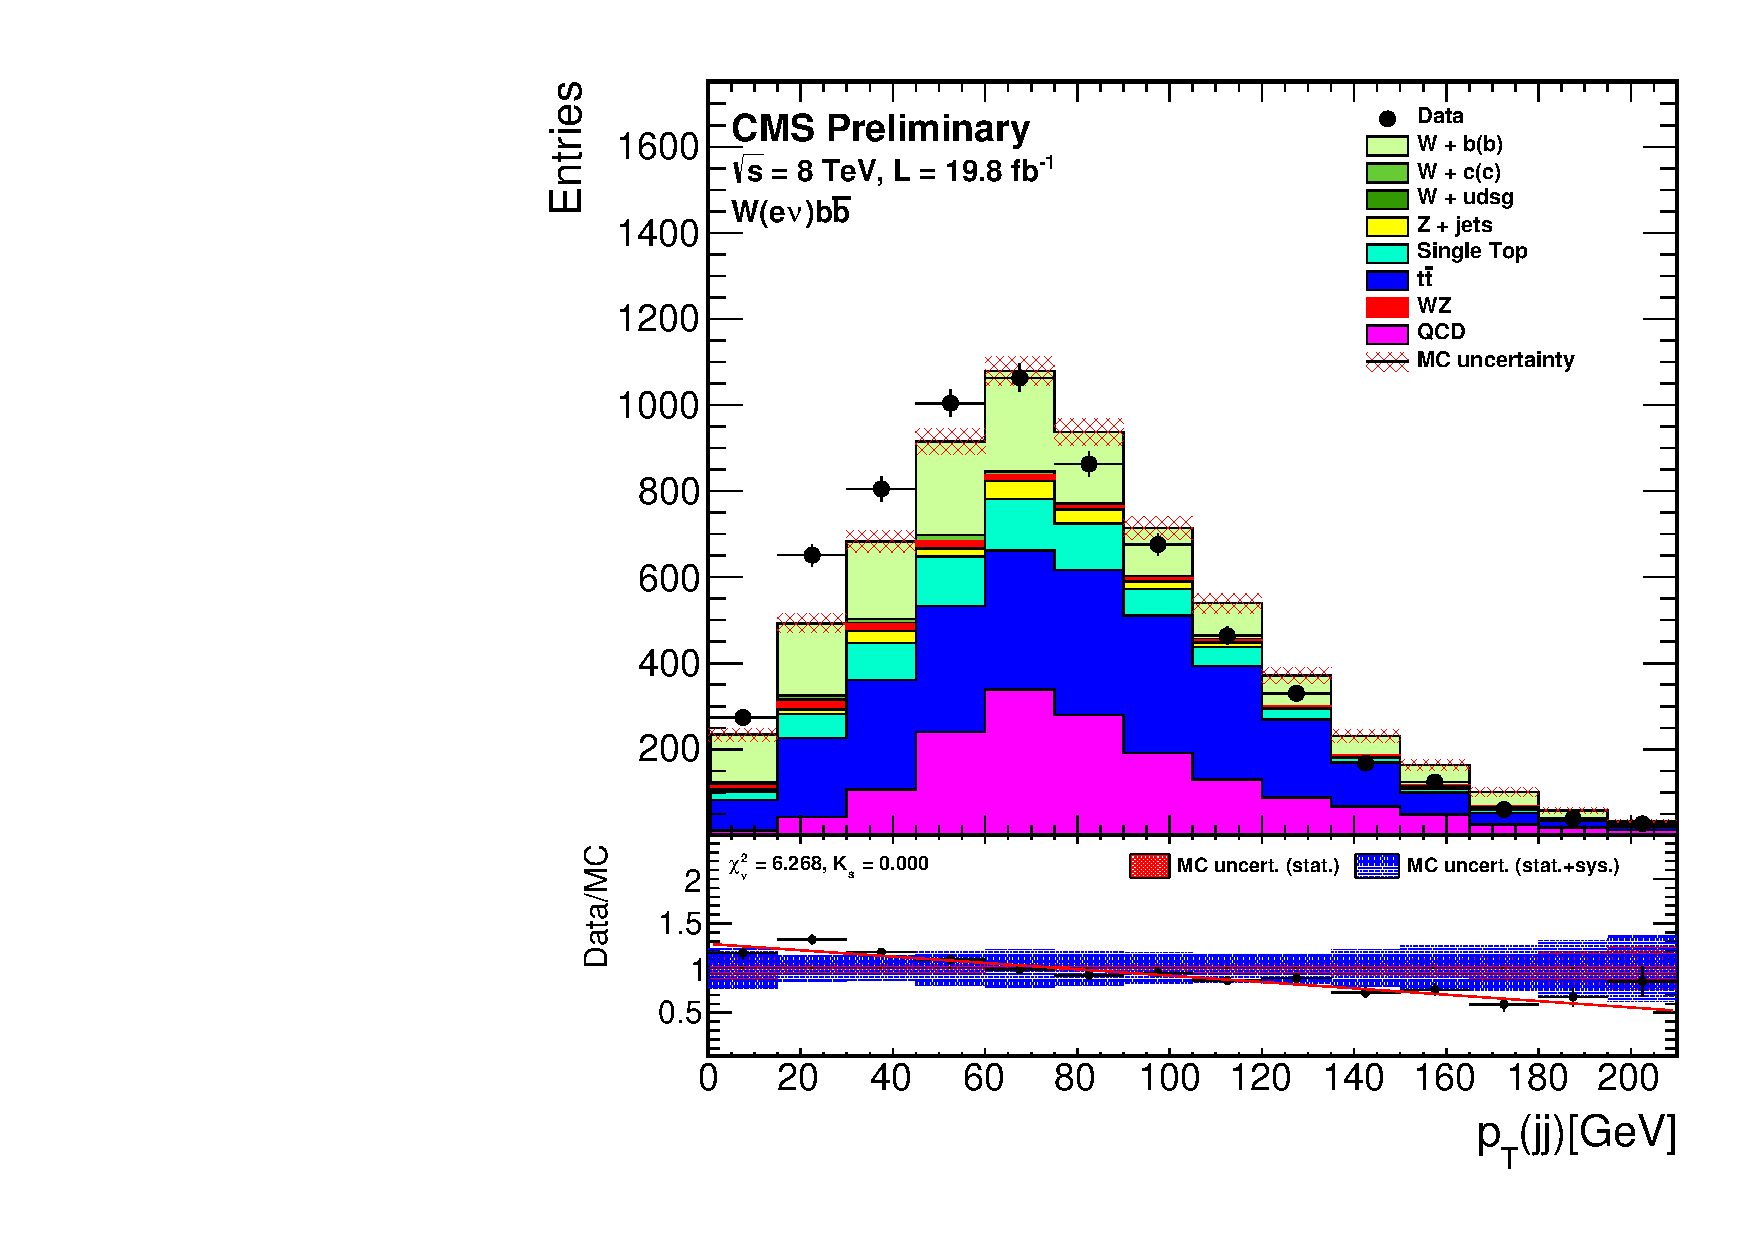
\includegraphics[width=0.48\textwidth]{Figures/Results/Electron/postfit/Wbb_H_pt_doQCD1.pdf}
		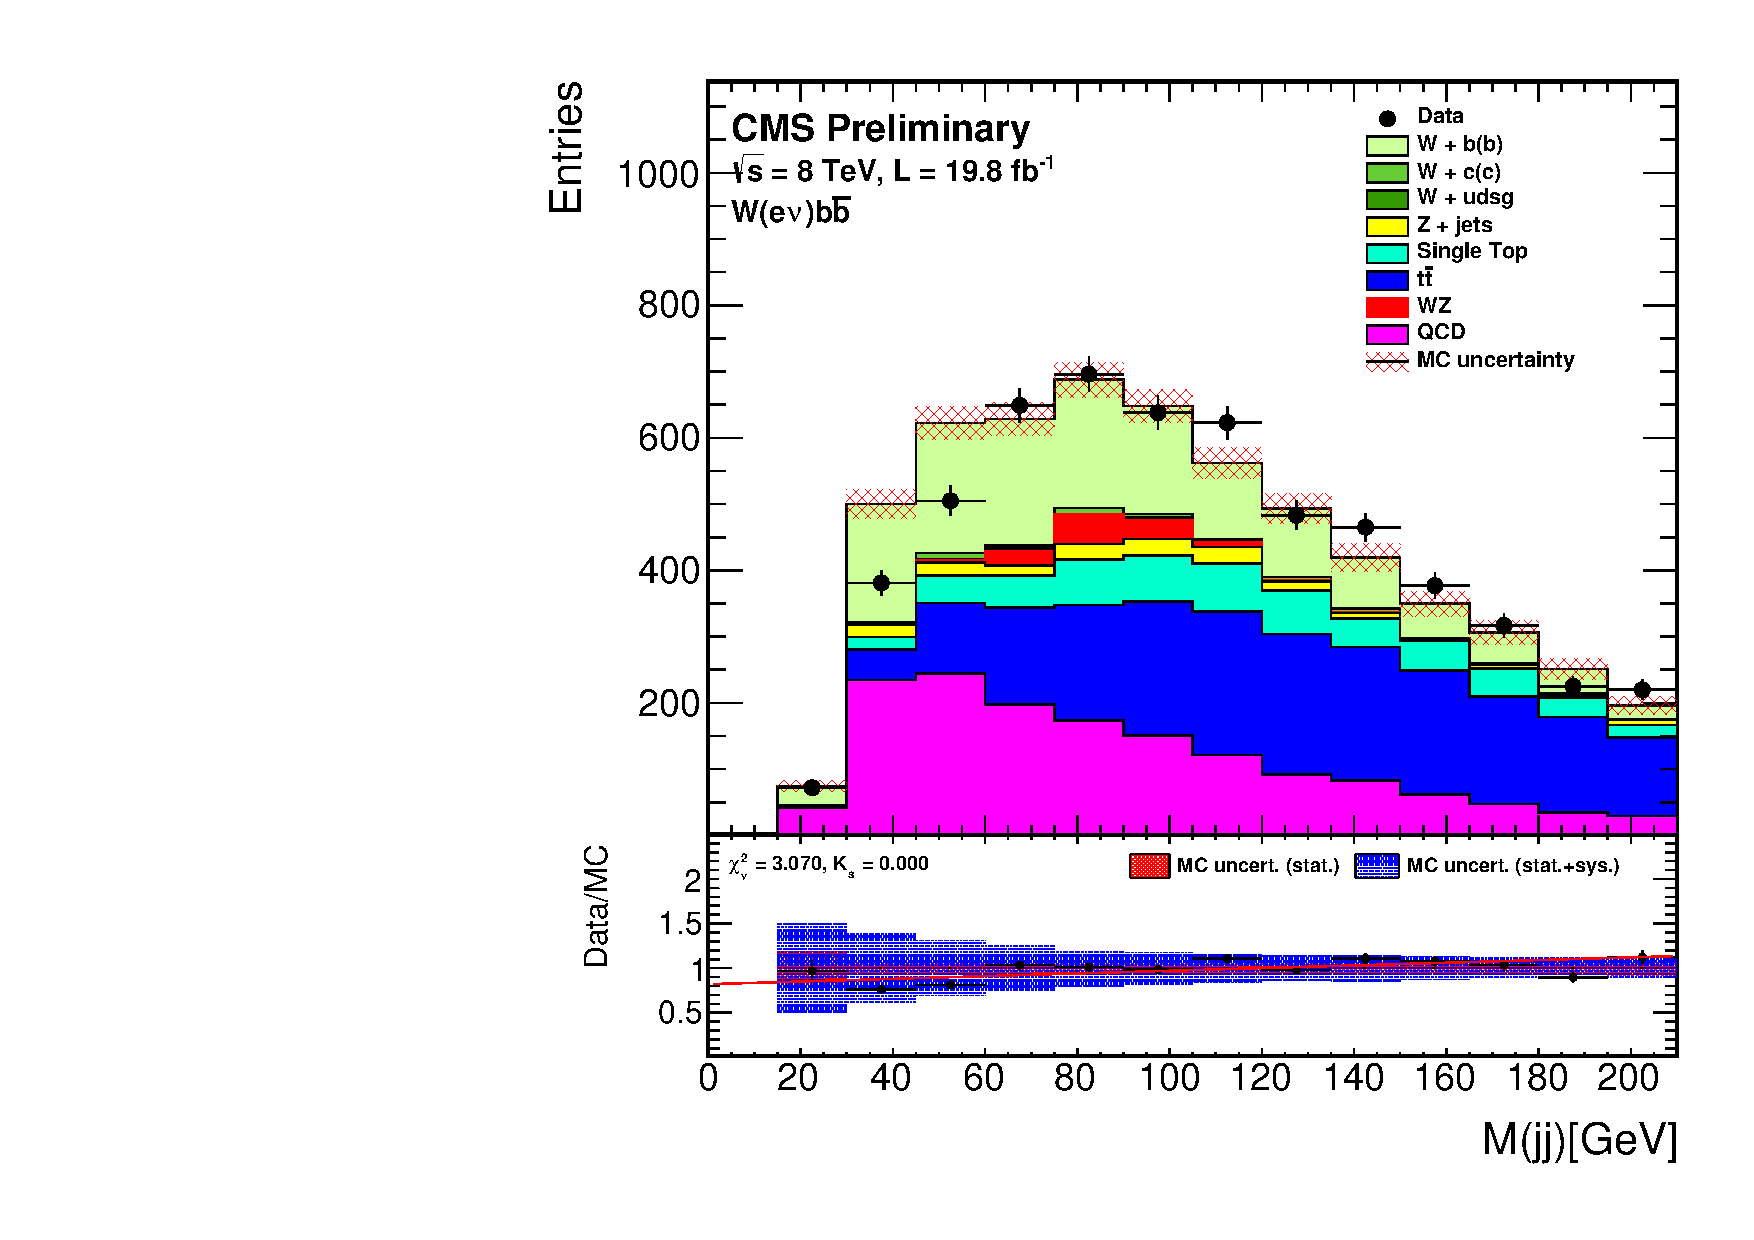
\includegraphics[width=0.48\textwidth]{Figures/Results/Electron/postfit/Wbb_H_mass_doQCD1.pdf}
		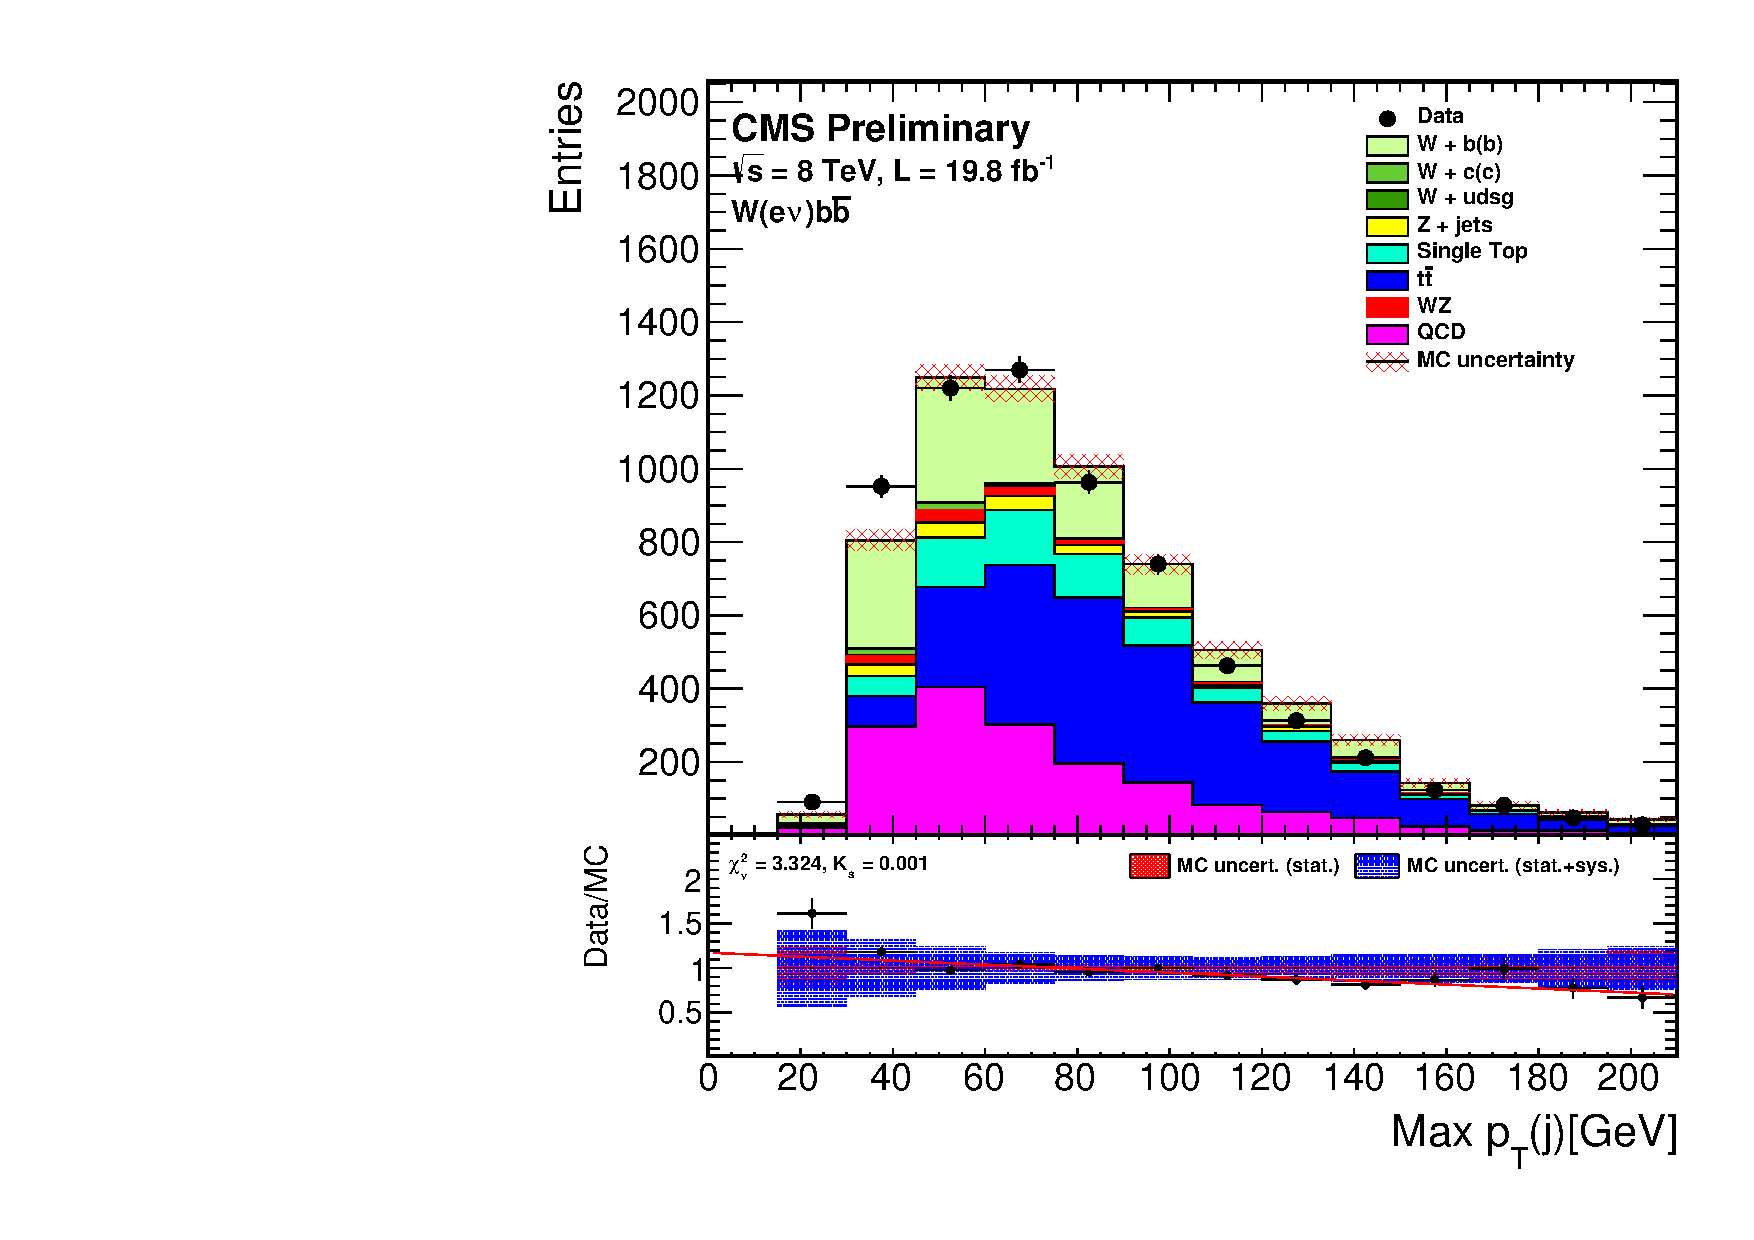
\includegraphics[width=0.48\textwidth]{Figures/Results/Electron/postfit/Wbb_max_hJet_pt_doQCD1.pdf}		
		%\rule{35em}{0.5pt}
	\caption{Electron channel distributions after the fit.}
	\label{fig:Wbb_postfit_ele}
\end{figure}

\subsection{Effects of the systematic uncertainties}
\label{sec:systEff}

Information about each source of systematic uncertainty together with the information whether just normalization or shape is included in the final fit is shown in table \ref{tab:systMu} for the muon channel and \ref{tab:systEle} for the electron channel. The tables also show the uncertainties on signal and background yields and the relative contribution to the signal strength uncertainty.
Due to correlations, the total systematic uncertainty is smaller that the quadrature sum of individual uncertainties. The last column shows the decrease in total systematic uncertainty when removing a specific source of uncertainty.

\begin{table}
\caption[Systematic uncertainties in the muon channel.]{Systematic uncertainty effect on the final yield is shown in the table together with the uncertainty on the signal and background yields and relative contribution to the signal strength uncertainty. }
\label{tab:systMu}
\begin{adjustbox}{width=\textwidth,center=\textwidth}
\begin{tabular}{ccccc} \hline \hline
&  & Event yield uncertainty &Individual contribution & Effect of removal  \\
Source & Type & range (\%) &  to $\mu$ uncertainty (\%) & on $\mu$ uncertainty (\%) \\ \hline 
b-tag efficiency & shape & 6.80 & 0.97 & 3.76\\
Lepton ID/Iso/Trig & shape & 0.57 & 0.27 & $<0.01$\\
Jet resolution & shape & 0.03 & $<0.01$ & 0.07\\
Jet energy scale & shape & 0.05 & 3.43 & 0.63\\
Unclustered MET & shape & 0.00 & $<0.01$ & 9.35\\
Muon energy scale & shape & 1.09 & 0.13 & 0.01\\
Luminosity & norm. & 2.60 & 0.67 & 0.02\\
Monte Carlo statistics & norm. & 0.75 & 3.63 & 10.10\\
\hline 
\end{tabular}
\end{adjustbox}

\end{table}

\begin{table}
\caption[Systematic uncertainties in the electron channel.]{Same as table \ref{tab:systMu} for the electron channel.}
\label{tab:systEle}
 \begin{adjustbox}{width=\textwidth,center=\textwidth}
\begin{tabular}{ccccc} \hline \hline
&  & Event yield uncertainty &Individual contribution & Effect of removal  \\
Source & Type & range (\%) &  to $\mu$ uncertainty (\%) & on $\mu$ uncertainty (\%) \\ \hline 
b-tag efficiency & shape & 6.80 & 1.01 & 2.13\\
lepton ID/iso/trigg & shape & 0.57 & 0.35 & 0.05\\
Jet resolution & shape & 0.03 & 0.02 & 0.24\\
Jet energy scale & shape & 0.05 & 0.30 & 3.71\\
Unclustered MET & shape & 0.00 & $<0.01$ & 1.15\\
Muon scale & shape & 1.09 & 0.15 & 0.24\\
Luminosity & norm. & 2.60 & 0.30 & 11.11\\
Monte Carlo statistics & norm. & 0.75 & 1.16 & 11.96\\
\hline 
\end{tabular}
 \end{adjustbox}

\end{table}

%\begin{figure}[htbp]
%	\centering
%		\includegraphics[width=0.8\textwidth]{Figures/Results/Muon/systPlots/MuMTstability_abo_5FS.pdf}
%		\includegraphics[width=0.8\textwidth]{Figures/Results/Muon/systPlots/MuMTstability_one_5FS.pdf}		
%	\caption{ABOONE}
%	\label{fig:systStability_mu}
%\end{figure}
%\begin{figure}[htbp]
%	\centering
%		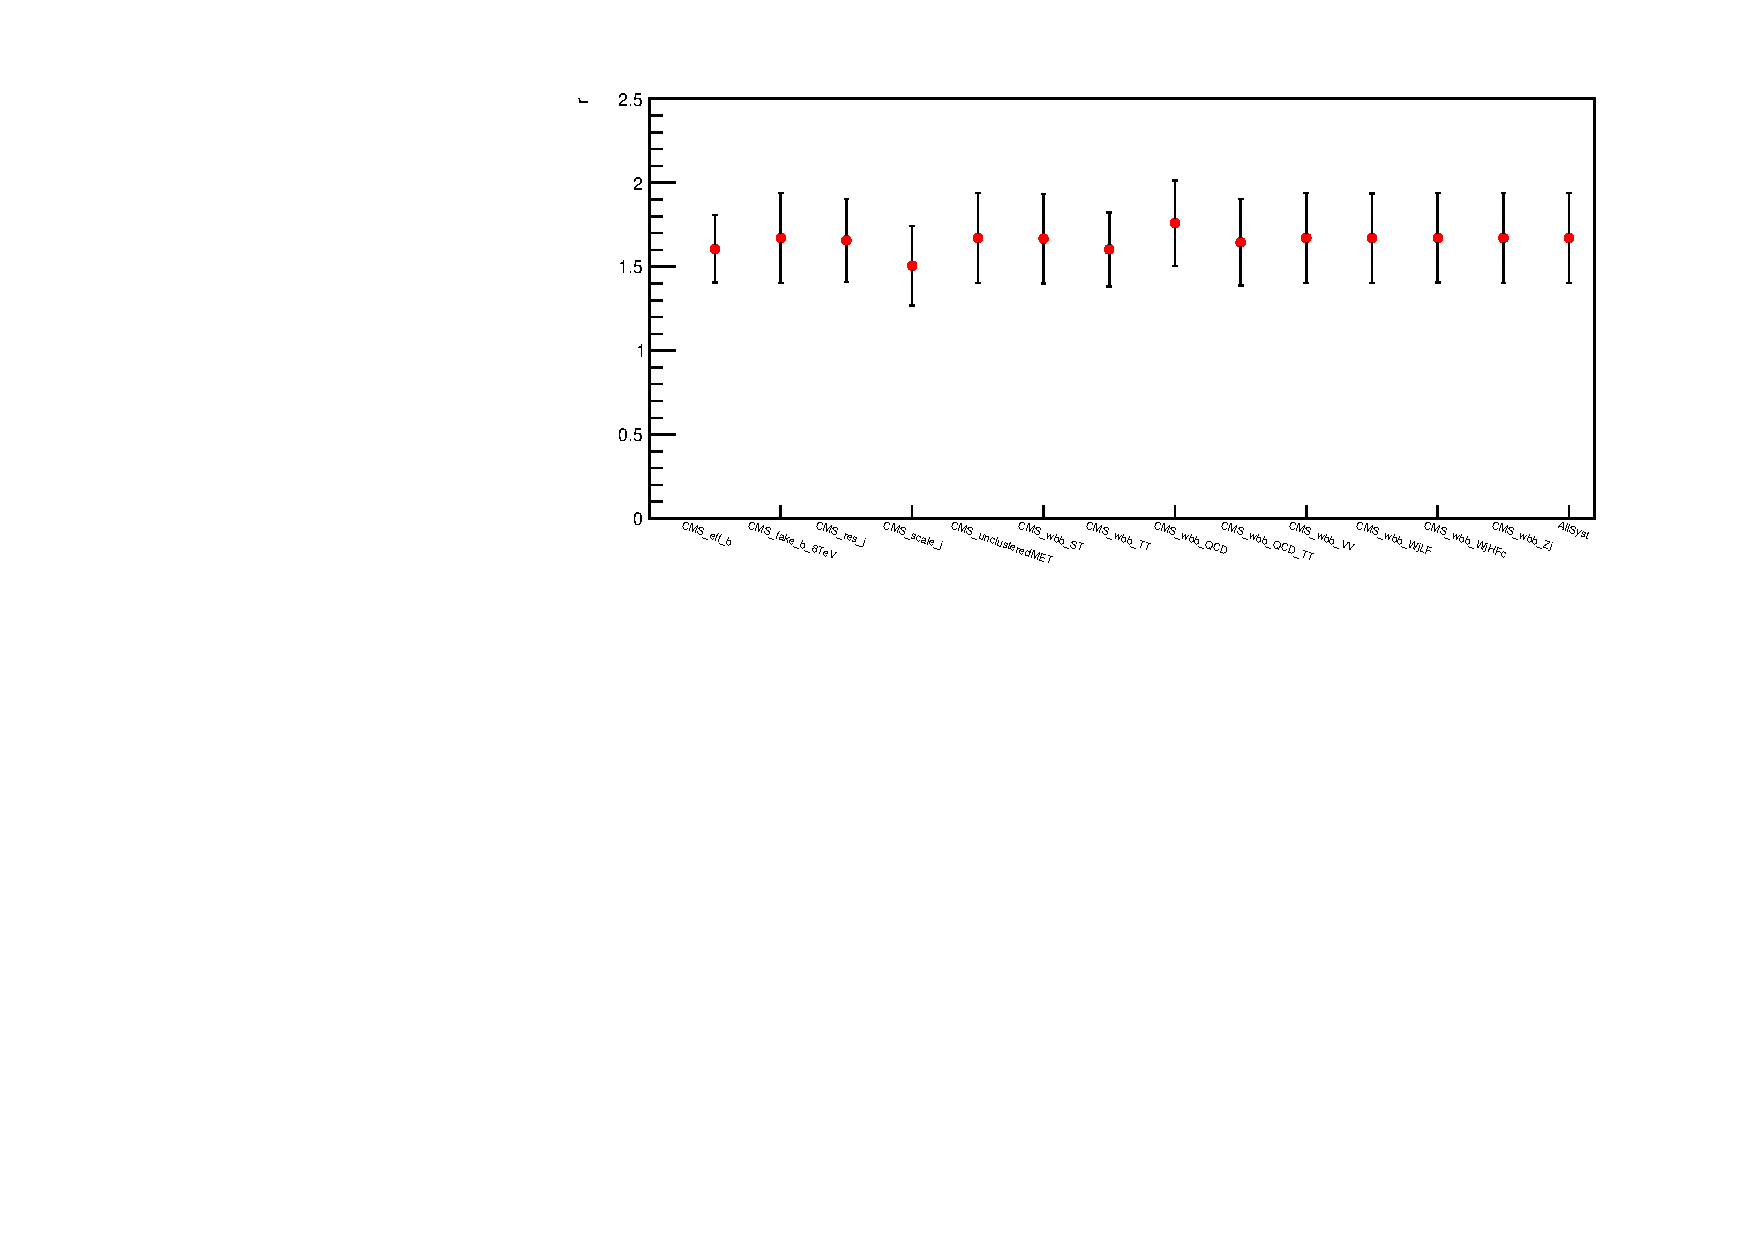
\includegraphics[width=0.8\textwidth]{Figures/Results/Electron/systPlots/EleMTstability_abo_5FS.pdf}
%		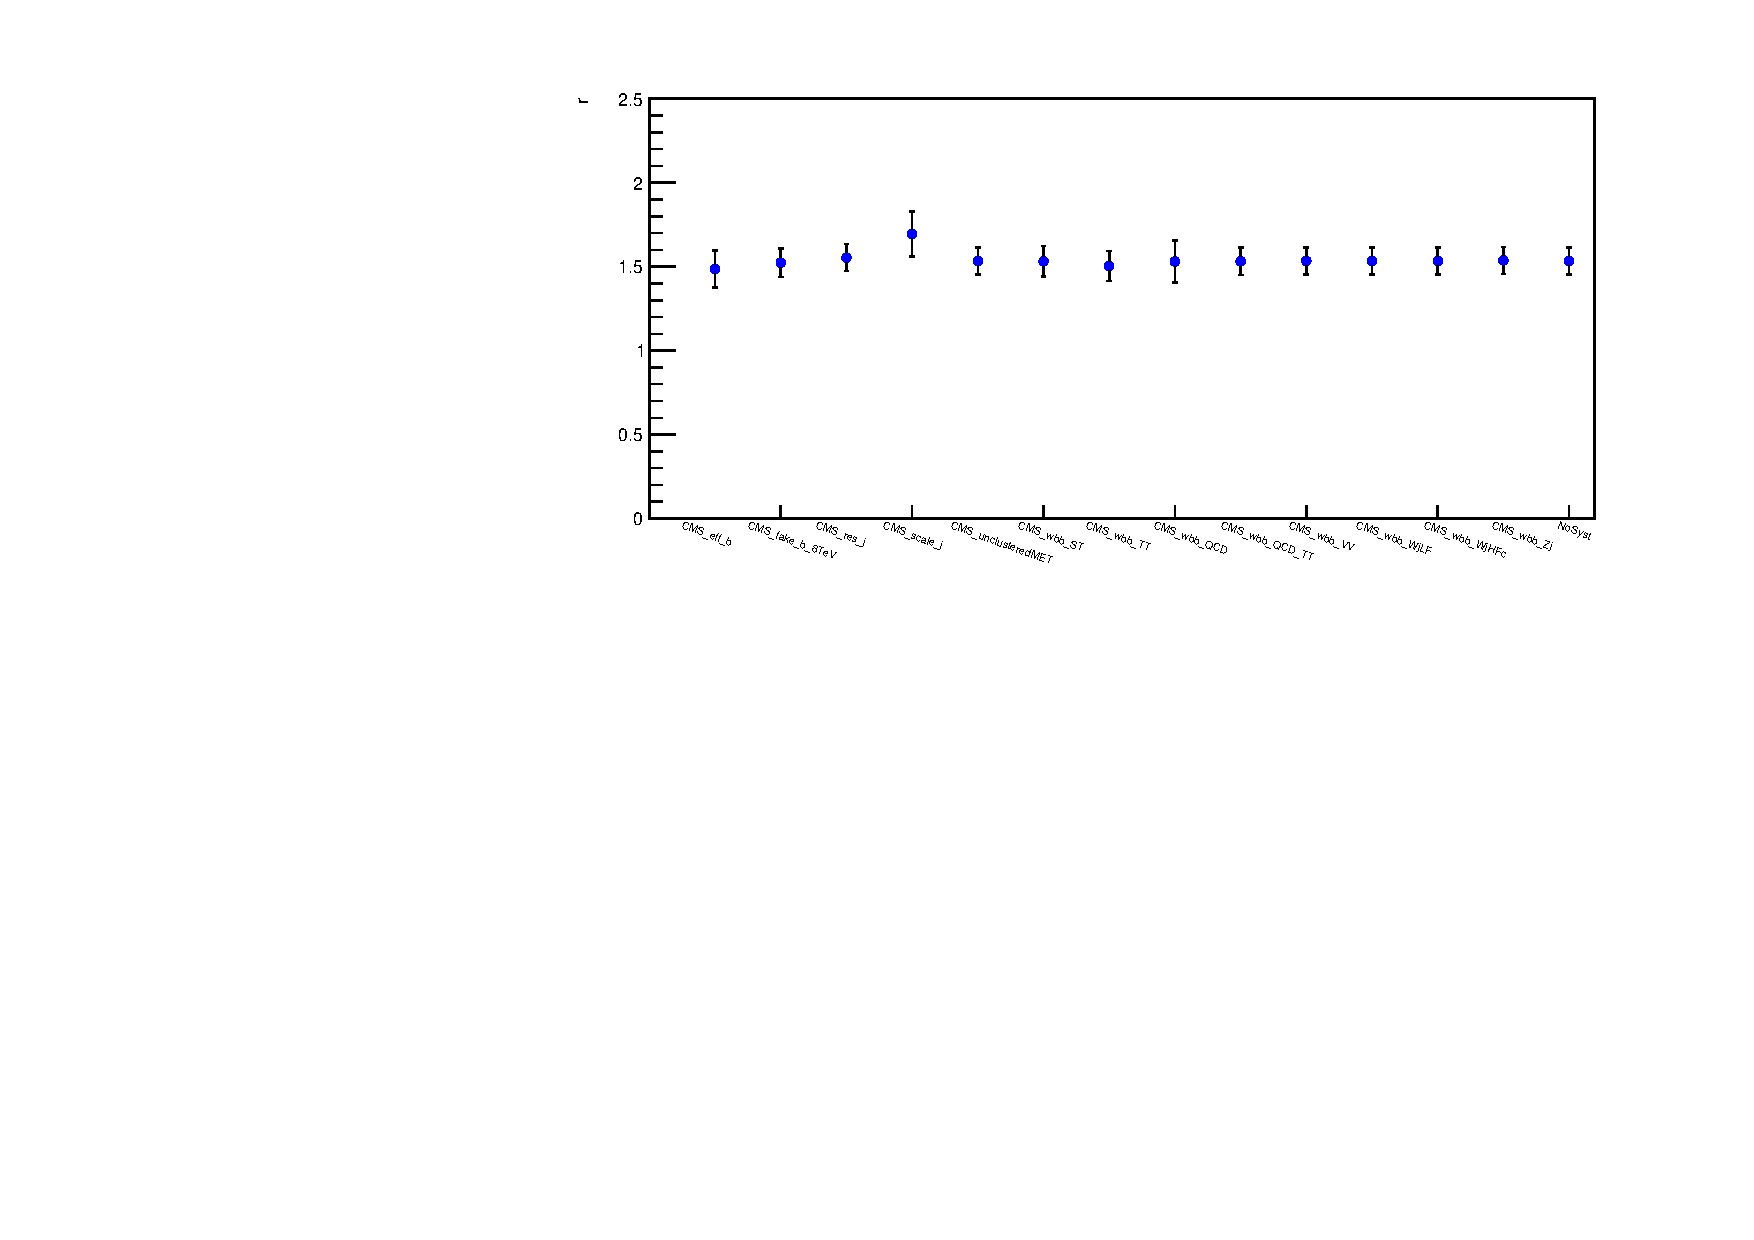
\includegraphics[width=0.8\textwidth]{Figures/Results/Electron/systPlots/EleMTstability_one_5FS.pdf}		
%	\caption{ABOONE}
%	\label{fig:systStability_ele}
%\end{figure}



\subsection{Tests of the fit stability}

Additional tests were performed in order to verify consistency of the obtained signal strength.
This was done by fitting different combinations of distributions in both signal region and $t\bar{t}$ control region.
Additional distributions include missing energy in the signal region and $t\bar{t}$ control region shown in figures \ref{fig:Wbb_prefit_muon} and \ref{fig:TT_CR} and invariant mass of third and fourth jet in $t\bar{t}$ control region. All used distributions show good agreement
in shapes between data and simulations making them suitable for the fit. Fitting procedure is performed in the muon channel only, as previously described.
Obtained signal strengths are summarized in Table \ref{tab:addFitTest} and are found to be consistent with the transverse mass fit.
\begin{table}[!htb]
\begin{center}
   \begin{tabular} {ccc} \hline\hline
   Fitted distribution (Wbb/$t\bar{t}$) & ~~~Signal Strength~~~ & ~~~~Yield Ratio~~~ \\
        \hline
        $M_T$/$M_T$                     &1.34$\pm$0.15  &1.55\\
        $M_T$/$E^{miss}_T$              &1.31$\pm$0.14  &1.52\\
        $M_T$/$M(j_3j_4)$               &1.35$\pm$0.16  &1.53\\
        $E^{miss}_T$/$M_T$              &1.43$\pm$0.21  &1.64\\
        $E^{miss}_T$/$E^{miss}_T$       &1.33$\pm$0.17  &1.53\\
        $E^{miss}_T$/$M(j_3j_4)$        &1.38$\pm$0.21  &1.55\\
   \hline\hline
   \end{tabular}
 \caption{UPDATE NUMBERS! - Signal strengths obtained by fitting different distributions. Signal strengths are found to be consistent with each other.}
\label{tab:addFitTest}
\end{center}
\end{table}

\subsection{Cross section measurement}

The inclusive cross section measurement was performed in the fiducial region corresponding to one lepton with $p_T>$30 GeV and $|\eta|<$2.1 and exactly two jets $p_T>$ 25 GeV and $|\eta|<$2.4. Jets are required to have at least one particle originating from a B hadron within a cone of 0.5 from the jet axis. The cross section was computed using the relation \ref{equ:xsec}, where the signal yields were obtained by multiplying the Wbb yield with the signal strength obtained from the fitting procedure for muon and electron channel, respectively. Acceptance and efficiency are taken from table \ref{tab:AE} and luminosity corresponds to 19.8 fb$^{-1}$. The measured cross sections are:
\begin{align*}
\sigma(pp\rightarrow W+bb)\times \mathcal{B}(W\rightarrow \mu\nu) = 0.66 \pm 0.03(\mathrm{stat.}) \pm 0.10(\mathrm{syst.})\\
\sigma(pp\rightarrow W+bb)\times \mathcal{B}(W\rightarrow e\nu) = 0.78 \pm 0.04(\mathrm{stat.}) \pm 0.13(\mathrm{syst.})
\end{align*}
The quoted systematic and statistical uncertainties take into account all previously described effects. However, these results are not taking into account the systematic effects on the acceptance and efficiency calculation of different choices for the parton distribution functions, or the effect of variation of factorization and renormalization scales. These effects were assessed in the previous measurements of Wbb process by the CMS experiment and contribute 10\% to the total cross section uncertainty \cite{Chatrchyan:2013uza}. The obtained cross section for electrons is somewhat higher than the one for muons but still within the systematic uncertainties.   

\subsection{Theoretical predictions and comparison with the measurement}

The theoretical prediction for the cross section defined in table \ref{tab:fiducial} was estimated using MCFM 6.8 in the massless five flavour scheme at NLO precision with factorization and renormalization scales set to the mass of the W boson. A hadronization correction factor $0.92\pm 0.01$ to extrapolate from the final-state particle jets to the parton-level cross section is estimated with MADGRAPH+PYTHIA. The obtained result is the following:
\begin{equation*}
\sigma_{TH}(pp\rightarrow W+bb)\times \mathcal{B}(W\rightarrow l\nu)=0.508\pm 0.001 \mathrm{stat.} \pm 0.005 \mathrm{PDF} \pm 0.029 \mathrm{scale} \pm 0.01 \mathrm{hadronization} \mathrm{\ pb}
\end{equation*} 
The statistical uncertainty associated to this result comes from the integration step of the calculation; the PDF and scale uncertainties have been estimated by repeating the calculation with different PDF sets and by varying the renormalization and factorization scales by a factor two with respect to the reference values ( M_W ).
\par The double parton scattering contribution was not taken into account during the theoretical calculation. However, it has been estimated following the procedure described in section \ref{sec:DPS} using the formula:
\begin{equation}
\sigma_{DPS} = \frac{\sigma_W \times \sigma_{bb}}{\sigma_{eff}}
\end{equation}
where $\sigma_W$ and $\sigma_{bb}$ are the corresponding single parton scattering cross sections for the production of the W boson and the production of b quark pair respectively. These cross sections were estimated for the same fiducial region as for the analysis and correspond to:
\begin{align*}
\sigma_{W} &= 4361 \pm 79 \mathrm{\ pb} \\
\sigma_{bb} &= 0.18 \pm 0.09 \mathrm{\ \mu b}.
\end{align*}
The inclusive cross section for the W boson production $\sigma_W$ is estimated with FEWZ \cite{Gavin:2012sy} at NNLO level. The total cross section for a pair of b quarks is estimated on a sample of events created with Madgraph and is accurate to LO precision, yielding a much larger associated uncertainty. The value of the effective cross section $\sigma_{eff}$ measured by the CMS is:
\begin{equation*}
\sigma_{eff}=20.7 \pm 6.6 \mathrm{\ mb}.
\end{equation*}   
The resulting contribution from double parton scattering to the Wbb cross section is:
\begin{equation*}
\sigma_{DPS}=0.40 \pm 0.02 \mathrm{\ pb}.
\end{equation*}
yielding the final Wbb cross section of:
\begin{equation*}
\sigma_{TH}(pp\rightarrow W+bb)\times \mathcal{B}(W\rightarrow l\nu) = 0.55 \pm 0.03 \mathrm{(theor.)} \pm 0.02 \mathrm{(DPS)} \mathrm{\ pb}.
\end{equation*}

The results for the cross section measurement obtained in this thesis are one standard deviation away from the theoretical predictions for the electron and the muon channel. 
%\begin{table}[!htb]
%\begin{center}
%   \begin{tabular} {r|l|l} \hline \hline
%\bf{W+bb} & \multicolumn{2}{c}{Fit Result: r = 1.34 $\pm$ 0.16}\\
%        Sample          & Prefit                & Postfit \\
%        \hline
%        W+bb            &879.7$\pm$23.2         &1350.0\\
%        W+cc            &35.5$\pm$8.2           &42.5\\
%        W+udscg         &19.7$\pm$6.9           &20.1\\
%        Z+jets          &122.5$\pm$17.3         &131.2\\
%        Single Top      &722.1$\pm$15.5         &833.0\\
%        T$\bar{T}$      &2338.6$\pm$11.1        &2676.7\\
%        VV              &106.4$\pm$2.6          &121.4\\
%        QCD             &249.3$\pm$14.9         &220.6\\
%        \hline
%        Total MC        &4473.9$\pm$39.4        &5426.1\\
%        \hline
%        Data&\multicolumn{2}{c}{5355.0$\pm$73.2}\\
%   \hline\hline
%   \end{tabular}
%\caption{Yields of MC samples before and after the fit.}
%\label{tab:fitYieldsJelena}
%\end{center}
%\end{table}
%
%
%
%
%

